\chapter{Literature Review}\label{chap:literature-review}

\textbf{TODO: reread}

As part of the problem awareness phase, the literature review summarises the relevant scientific literature related to the topics of this thesis.
It lays the groundwork for answering to the research questions.
Initially, Sec.~\ref{sec:research-collaboration} discusses the definition and importance of research collaboration and methods for finding potential research collaborators.
Sec.~\ref{sec:knowledge-graphs} provides an overview of knowledge graphs, from theoretical aspects to real-world applications.
Existing knowledge graphs and ontologies in the research field are also described.
Sec.~\ref{sec:large-language-models} briefly provides an overview of \glspl{llm}, applications of these technologies with their advantages and limitations.
Finally, Sec.~\ref{sec:recommender-systems} explains recommender systems, particularly existing recommendation systems in the search domain and \gls{rag}-based recommendation systems.
%
\section{Research Collaboration}\label{sec:research-collaboration}
\subsection*{Definition and Importance of Research Collaboration}
\textcite{Bozeman2014} define research collaboration as the process in which individuals pool their skills, knowledge, and resources to generate new scientific insights and address complex challenges.
It has been described as a social process that combines human capital, such as formal training and technical skills, with social capital, including networks and collaborative relationships, to advance knowledge creation \cite{Bozeman2014}.
This collaboration often takes place within the framework of ``team science'', where interdisciplinary teams work collectively to tackle multifaceted problems that surpass the scope of single-discipline research.
Within research collaboration, the goals can range from knowledge-based objectives, such as publishing academic articles and creating educational resources, to property-based outcomes, including patents and commercial technologies.

Co-authorship is frequently used as a tangible indicator of collaboration, though it only captures a fraction of the collaborative efforts that occur in scientific work.

Boundary-spanning collaborations, such as those crossing institutional, disciplinary, or sectoral lines, are particularly crucial for addressing global challenges but require careful alignment of goals and effective communication to overcome cultural and operational differences.

Despite its significant benefits, research collaboration is often impeded by challenges such as disciplinary silos, communication barriers, and logistical constraints.
As collaboration becomes increasingly essential in the era of team science and global research, understanding these dynamics is critical for fostering effective partnerships and advancing scientific discovery.

\textcite{KATZ19971} define the term ``research collaboration'' refers to the process where researchers from various disciplines, institutions, or regions work together toward shared objectives.
It plays a critical role in advancing scientific knowledge, addressing complex challenges, and fostering innovation.
Collaborative efforts enable the pooling of diverse expertise, resources, and perspectives, which are essential for tackling interdisciplinary problems \cite{KATZ19971}.
The increasing prevalence of co-authored publications and large-scale projects underscores the importance of collaboration in modern academia \cite{Adams2012}.

\subsection*{Methods to Find Research Collaborators}
Identifying suitable collaborators is a foundational step in establishing successful research partnerships.
Finding a potential research collaborator often relies on various methods, with personal and professional networking being among the most prominent.
According to \textcite{KATZ19971}, traditional approaches like conferences, workshops, and seminars provide researchers with opportunities to establish connections and build trust, which is critical for reducing the transaction costs of collaboration and enhancing its overall effectiveness.
These face-to-face interactions create a foundation for partnerships by fostering mutual understanding and shared interests, especially in multidisciplinary fields \cite{Bozeman2014}.

Institutional and organizational connections also play a significant role in facilitating collaborations. Universities and research centers often promote partnerships through formal agreements or structured programs, giving researchers access to a broader network of professionals and shared resources. These institutional linkages help bridge gaps between disciplines or organizations, enabling researchers to leverage collective expertise and infrastructure.

Trust and social capital are fundamental factors in initiating and sustaining collaborations. Collaborations often emerge from prior acquaintance or existing professional relationships, where trust reduces the perceived risks and uncertainties involved in working together. This trust is particularly vital in interdisciplinary or inter-institutional collaborations, where differences in methodologies, goals, or organizational cultures might otherwise hinder progress \cite{Bozeman2014}.

Additionally, recommendations from colleagues, mentors, or supervisors often serve as effective means of identifying potential collaborators.
These recommendations draw on the existing trust and knowledge of the recommender, providing a reliable basis for collaboration \cite{Bozeman2014}.

Ultimately, the success of research collaboration depends on key factors such as the alignment of research goals, complementary expertise, effective communication, and the ability to navigate cultural or disciplinary differences.
By leveraging these methods and addressing these factors, researchers can establish productive and enduring partnerships \cite{Bozeman2014}.

Digital platforms have increasingly become essential tools for finding collaborators. Online academic networks, citation databases, and digital communities allow researchers to search for potential collaborators based on shared research interests, publication records, or complementary expertise. These platforms have expanded the reach of collaborations, making it easier for researchers to connect globally and explore new opportunities.
However, these methods often require researchers to actively seek and evaluate potential collaborators, which can be time-intensive and subjective.
%
\section{Knowledge Graphs}\label{sec:knowledge-graphs}
\glspl{kg} have came up as a key technology in the field of data management and \gls{ai}, enabling sophisticated data integration, retrieval and analysis.
This section provides an in-depth overview of \glspl{kg}, their theoretical foundations, practical applications and recent advances.

\subsection*{Theoretical Foundations of Knowledge Graphs}
\subsubsection*{Definition and Structure}
\glspl{kg} are directed graph-based data structures that represent real-world entities and their interrelations, providing a way to model complex domains and their underlying semantics.
A \gls{kg} consists of nodes (also called entities) and edges (also called relationships), forming a network of interconnected information.
This structure allows \glspl{kg} to capture rich contextual information and provide a semantic framework for data \cite{Hogan2021}.
In other words, a \gls{kg} refers to a semantic network graph which is consisted of diverse entities, concepts, and relationships.
It is used to formally describe various things and their associations in the real world.
\glspl{kg} are generally represented in triples $\gls{kg}=\{\mathnormal{E,R,F}\}$, where:
\begin{itemize}
    \item $E$ represents the entity set $\{\mathnormal{e_1, e_2, ... ,e_E} \}$, and the entity $e$ is the most basic element in the \gls{kg}, referring to the items that exist objectively and can be distinguished from each other.
    \item $R$ represents the relation set $\{\mathnormal{r_1, r_2, ... ,r_R}\}$, and the relation $r$ is an edge in the \gls{kg}, representing a specific connection between different entities.
    \item $F$ represents the fact set $\{\mathnormal{f_1,f_2, ... ,f_F}\}$, and each $\mathnormal{f}$ is defined as a triple $(\mathnormal{h,r,t}) \in \mathnormal{f}$, in which $\mathnormal{h}$ denotes the head entity, $\mathnormal{r}$ stands for the relationship, and $\mathnormal{t}$ indicates the tail entity.
\end{itemize}

The \gls{kg} in Fig.~\ref{fig:kg-example-albert-einstein} visually represents some relationships and attributes associated with Albert Einstein.
At the center of the graph is ``Albert Einstein'', from which several connections extend.
One connection indicates that he was ``born in'' Germany.
Another connection shows his ``occupation'' as a ``Theoretical Physicist''.
This occupation is further connected to ``Physicist'' as a ``kind of'' category, indicating that a theoretical physicist is a type of physicist.
The graph also shows that a physicist ``practices'' physics.
Additionally, it highlights that Albert Einstein ``developed'' the ``Theory of Relativity'', which is shown as a ``branch of'' physics.
The graph effectively maps out key aspects of Albert Einstein's background, profession, and contributions to science.

\begin{figure}[htbp]
    \centering
 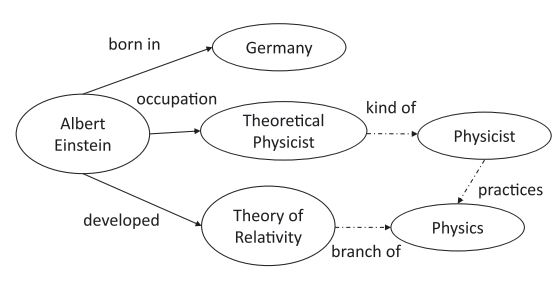
\includegraphics[width=.7\textwidth]{figures/literature-review/kg-example-albert-einstein.png}
     \rule{35em}{0.5pt}
    \caption{An example of \acrlong{kg} (\textcite{Chaudhri2022})} 
 \label{fig:kg-example-albert-einstein}
\end{figure}

\subsubsection*{Ontologies and Semantic Web Technologies}
An ontology is a formal representation of knowledge in a domain, specifying the concepts, relationships, and constraints that exist within that domain. The term ``ontology'' can be used to the shared understanding of some domain of interest \cite{Uschold1996}.
Ontologies play a critical role in defining the schema and semantics of \glspl{kg}. They specify the types of entities, relationships, and constraints, thereby providing a formalized structure for the data. The Semantic Web technologies, particularly the \gls{rdf} and the \gls{owl}, are fundamental to the development and functioning of \glspl{kg} \cite{Antoniou2008}.
\\\gls{rdf} is a standard model for data interchange on the web.
\gls{rdf} is a part of the \gls{w3c}'s Semantic Web activity and provides a model for data interchange on the Web.
It uses triples $\langle subject,predicate,object \rangle$ to represent information, providing a flexible and extensible framework for creating and managing \glspl{kg} \cite{Cyganiak14RCA}.
The subject is the resource being described, the predicate is the property or characteristic of the subject, and the object is the value of the property, that can be literals, which are concrete data values such as strings, numbers, or dates.
\gls{rdf} uses \glspl{uri} to uniquely identify subjects and predicates, ensuring that resources are globally identifiable.
\gls{rdf} can be serialized in various syntaxes, including \gls{rdf}/XML, Turtle, N-Triples, and JSON-LD. \gls{rdf}/XML is the original \gls{rdf} syntax using XML to represent \gls{rdf} triples. Turtle is a more human-readable syntax for \gls{rdf} data, concise and easier to write and read compared to \gls{rdf}/XML. N-Triples is a plain text format for encoding \gls{rdf} triples, useful for streaming data or simple data exchange. JSON-LD is a JSON-based format to serialize Linked Data, designed to be easy to use and integrate with existing JSON-based systems.

\gls{rdfs} is a semantic extension of \gls{rdf} that provides mechanisms to describe groups of related resources and the relationships between these resources. It allows for defining classes, which are categories of resources; properties, which are relationships between resources; and hierarchies, enabling inheritance.
\gls{rdf} is widely used in various domains, including the Semantic Web, where it enables the creation of a web of data with meaning, allowing machines to understand and process web content; \glspl{kg}, powering large-scale graph-based data structures used by organizations like Google and Amazon \cite{Kejriwal2022}; data integration, integrating data from disparate sources by providing a common data model; and ontology engineering, defining and using ontologies to model domain knowledge.

The \gls{owl} standard is a \gls{w3c} technology for defining and using web ontologies, enhancing \gls{rdf} by offering greater expressiveness for complex information. \gls{owl} ontologies consist of classes, properties, and individuals, enabling detailed descriptions of relationships and characteristics. It supports complex class expressions, including logical operators and restrictions like cardinality and property constraints.
\gls{owl} is used to explicitly represent the meaning of terms in vocabularies and the relationships between those terms. It enables more complex and expressive representations compared to \gls{rdfs} \cite{Deborah2004}.
\gls{owl} is used in knowledge management, information integration, and semantic search, providing a common framework for understanding and integrating data. It promotes interoperability and the creation of semantically rich, interconnected web data.

\subsubsection*{Query Languages}
\gls{sparql} is the standard query language for retrieving and manipulating data stored in \gls{rdf} format.
This query language is used to retrieve data from the GraphDB\footnote{\url{https://www.ontotext.com/products/graphdb/}} database.
It allows users to write complex queries to extract specific information from a \gls{kg}, making it a powerful tool for data analysis and knowledge discovery \cite{Jorge2009}.
It allows users to query \gls{rdf} data by specifying patterns of triples and to update \gls{rdf} data by inserting, deleting, and modifying \gls{rdf} triples. \gls{rdf} is a foundation for Linked Data, which involves interlinking data across the web using \glspl{uri} and \gls{rdf}. This enables the creation of a web of data that can be easily connected and queried.

Cypher is another query language for graph databases, such as Neo4j\footnote{\url{https://neo4j.com}}, that allows users to interact with graph data using a pattern-matching syntax. Cypher queries are used to traverse the graph, retrieve specific patterns, and perform operations on the data \cite{Francis2018}.
Cypher supports complex queries involving multiple nodes and relationships, aggregation, sorting, and limiting results. It also provides functions for working with strings, numbers, dates, and collections, as well as support for subqueries and variable-length paths.
Cypher is widely used for graph analytics, network analysis, and data exploration, enabling users to easily express complex graph traversals and operations. It leverages Neo4j's indexing and optimization capabilities to ensure efficient execution of queries, making it a powerful tool for working with connected data.

\subsection*{Applications of Knowledge Graphs}

\subsubsection*{General Applications}
\glspl{kg} have been adopted across various domains due to their ability to integrate heterogeneous data sources, provide semantic context, and enable advanced querying and reasoning.
According to \textcite{Kapanipathi2020}, in healthcare \glspl{kg} are used to integrate patient records, clinical trials, research data, and medical ontologies, enabling personalized medicine and decision support systems. They help in identifying relationships between diseases, treatments, and patient outcomes.
\\Financial institutions leverage \glspl{kg} to connect data from various sources, such as market data, regulatory information, and customer transactions. This integration facilitates risk management, fraud detection, and compliance monitoring \cite{Tchechmedjiev2019}.
\\In e-commerce, \glspl{kg} enhance product recommendation systems by linking customer preferences, purchase history, and product information. They enable more personalized and relevant recommendations, improving customer satisfaction and sales \cite{Zhang2021}.

In compliance with \textcite{Zou2020}, Fig.~\ref{fig:kg-application-fields} shows a mind map illustrating the main applications of knowledge graphs. It divides the applications into five main categories: question answering, recommendation systems, information retrieval, domain-specific applications and other applications.

\begin{figure}[htbp]
    \centering
 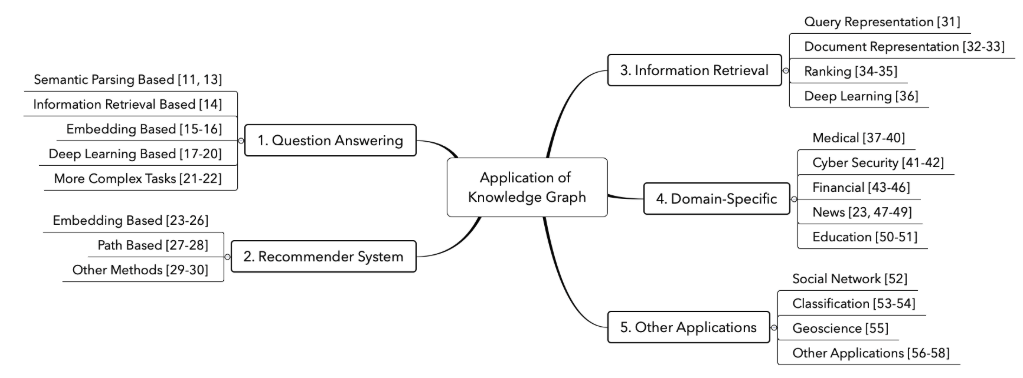
\includegraphics[width=\textwidth]{figures/literature-review/kg-application-fields.png}
     \rule{35em}{0.5pt}
    \caption{Application of \acrlongpl{kg} (\textcite{Zou2020})} 
 \label{fig:kg-application-fields}
\end{figure}

With regard to question answering, methods based on semantic parsing, methods based on information retrieval, methods based on embedding, methods based on \gls{dl} and more complex tasks are included.
\glspl{kg} significantly enhance search engines by providing semantic search capabilities. They enable the understanding of user queries in context, allowing for more accurate and relevant search results. Google's Knowledge Graph is a prominent example, enhancing search results with information about entities and their relationships \cite{singhal2012introducing}.
Recommender systems are classified into embedding-based methods, path-based methods and other methods. Information retrieval includes query representation, document representation, ranking and \gls{dl}. Domain-specific applications include medicine, computer security, finance, news and education.
Within enterprises, \glspl{kg} are used to manage and utilize internal knowledge effectively. They integrate data from different departments, such as human resources, finance, and operations, providing a unified view of the organization's information. This integration supports decision-making, collaboration, and innovation \cite{pujara2013knowledge}.
Other applications include social networks, classification, geosciences and various other applications.


\subsection*{Recent Advancements in Knowledge Graphs}

\subsubsection*{Integration with Machine Learning}
Recent research has focused on integrating \glspl{kg} with \gls{ml} and \gls{dl} techniques to enhance their capabilities and applications. These integrations have led to significant advancements in various areas, including \gls{nlp}, recommendation systems, and predictive analytics.

\glspl{kge}: \gls{kge} techniques represent entities and relationships in a continuous vector space, enabling the use of \gls{ml} algorithms for tasks such as link prediction, entity classification, and clustering. Popular methods include TransE \cite{Bordes2013}, TransH \cite{Wang2014}, and TransR \cite{Lin2015}, each providing different ways to model relationships in the embedding space \cite{Wang2017}.

\glspl{gnn}: \glspl{gnn} are \gls{dl} models designed to operate on graph-structured data. They leverage the relational nature of graphs to perform tasks such as node classification, link prediction, and graph classification. \glspl{gnn} have been successfully applied to enhance the capabilities of \glspl{kg} in various domains \cite{Wu2021}.

\subsubsection*{Natural Language Processing and Question Answering}
\glspl{kg} have been instrumental in advancing \gls{nlp} applications, particularly in question answering systems. By providing structured and semantically rich information, \glspl{kg} enable systems to understand and generate human language more effectively.
\glspl{kg} support question answering systems by enabling them to retrieve and reason over structured data.
These systems can answer complex queries by traversing the graph and applying logical inferences based on the relationships between entities \cite{Yasunaga2021}.
\glspl{kg} enhance text analysis and semantic search by providing contextual information about entities mentioned in the text.
This contextual understanding improves the accuracy of information retrieval and the relevance of search results \cite{Fernandez2011}.

\subsection*{Well-Known Knowledge Graphs and Ontologies in Research Field}
Well-known \glspl{kg} and ontologies have significantly influenced the research field by providing structured representations of knowledge that facilitate data integration, retrieval, and analysis.
One prominent example was the \gls{mag}, a comprehensive dataset that mapped scholarly publications, authors, institutions, and topics, enabling advanced research trend analysis and collaboration discovery \cite{Wang2020}.
Although \gls{mag} was discontinued in 2021 as Microsoft shifted its focus to supporting open academic initiatives, its legacy lives on through platforms like OpenAlex, a successor to \gls{mag} that serves as an open-source resource connecting entities such as authors, publications, and journals with detailed metadata \cite{priem2022}.

\begin{figure}[htbp]
    \centering
 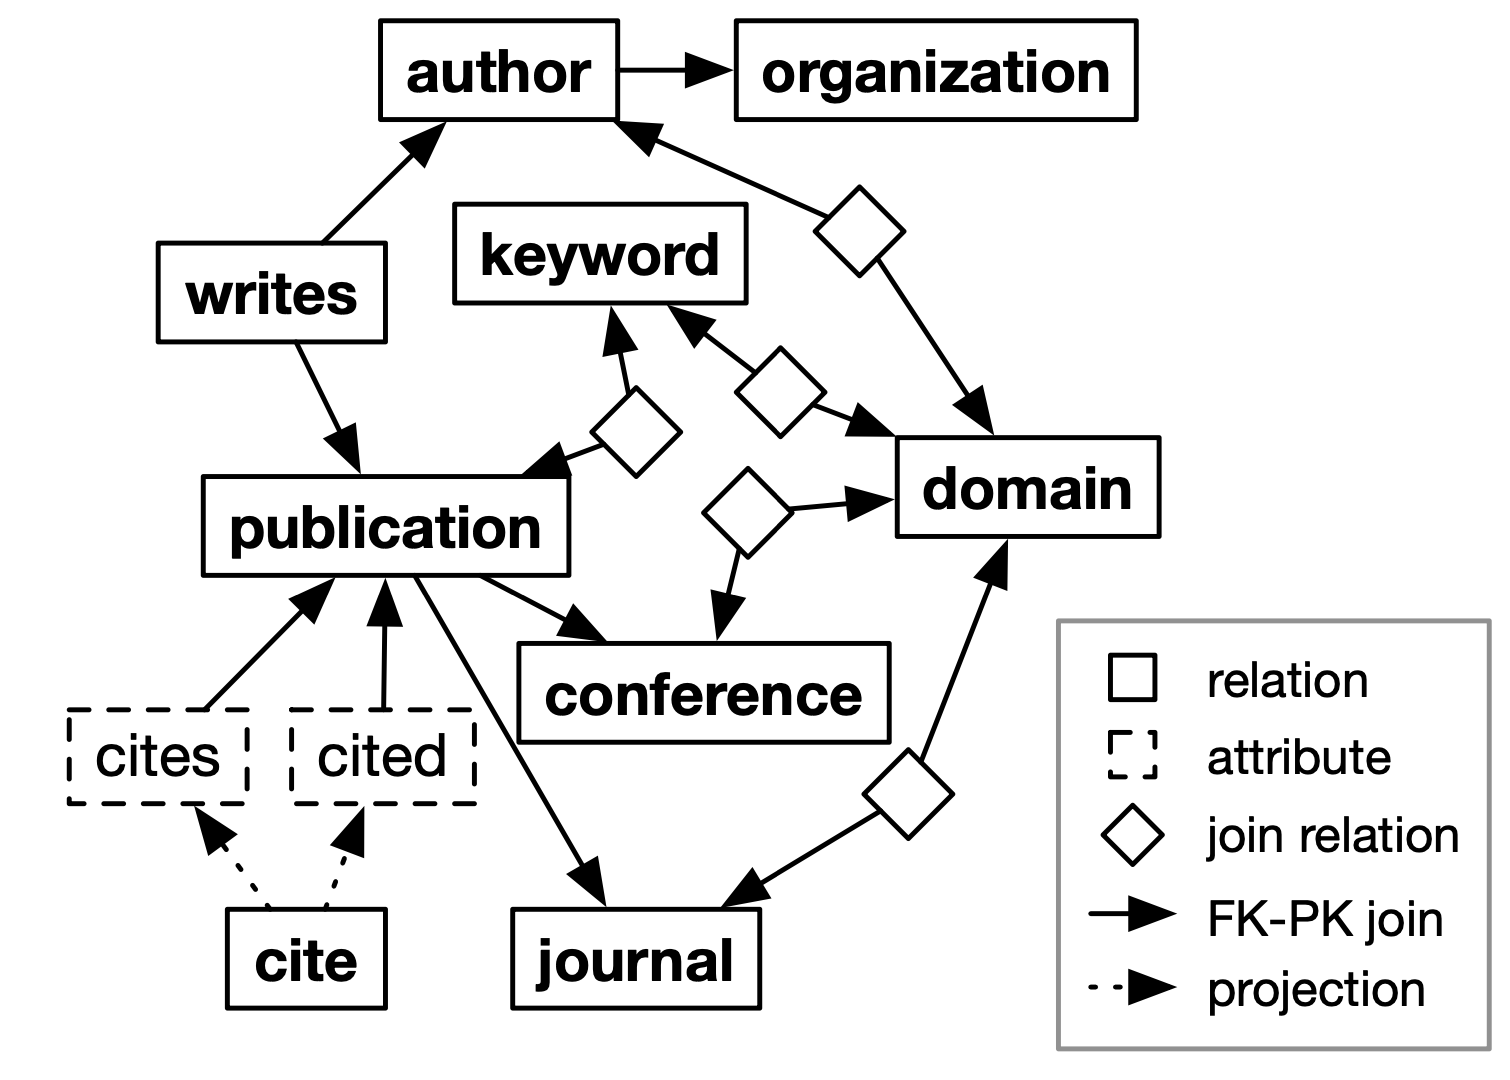
\includegraphics[width=0.8\textwidth]{figures/literature-review/mag-schema.png}
     \rule{35em}{0.5pt}
    \caption{A simplified version of the \gls{mag} Search database's schema (\textcite{Baik2019})} 
 \label{fig:mag-schema}
\end{figure}

Another essential resource is the the \gls{s2ag}, developed by the Allen Institute for \acrlong{ai}, represents one of the most extensive and advanced knowledge graphs in the research domain \cite{S2AG}.
\gls{s2ag} contains over 205 million publications, 121 million authors, and nearly 2.5 billion citation edges, making it a powerful resource for understanding and analyzing academic networks.
By integrating metadata from sources such as Crossref, PubMed, and Unpaywall, and processing nearly 60 million full-text publications, \gls{s2ag} enables rich insights into scholarly communication.
The data is accessible through public APIs and downloadable snapshots, fostering applications in natural language processing, citation analysis, and research trend discovery.
\gls{s2ag} exemplifies the potential of \glspl{kg} to address information overload by enabling efficient discovery of relevant research literature.
Its availability as an open resource highlights the growing emphasis on open science and collaborative innovation in the academic community.

Wikidata is a collaboratively edited \gls{kg} that serves as a centralized data repository for structured information across various domains, supporting Wikimedia projects like Wikipedia and numerous external applications \cite{Wikidata2014}.
Introduced in 2012 by the Wikimedia Foundation, Wikidata provides a platform where entities, such as people, places, events, and concepts, are represented as items with unique identifiers.
These items are described using statements, which consist of properties and values, forming a triple-based structure similar to other semantic web technologies.
One of the most distinguishing features of Wikidata is its adherence to the principles of \gls{lod}.
It allows the integration with other \glspl{kg} and ontologies by supporting globally recognized identifiers, such as \glspl{doi}, \glspl{orcid}, and \gls{viaf} IDs, and linking to external datasets.
This capability makes it a valuable resource for connecting fragmented knowledge across the web.
The Wikidata \gls{kg} is highly dynamic and continuously enriched by a global community of contributors and automated tools like bots.
Its multilingual support ensures accessibility to a diverse audience.
Applications of Wikidata include natural language processing, recommendation systems, semantic search, and research in \gls{ai}.
Due to its openness, flexibility, and integration capabilities, Wikidata is increasingly being adopted as a foundational resource for creating and enriching domain-specific knowledge graphs, supporting scholarly projects, and powering data-driven insights.

Furthermore, the \gls{orkg} offers a dynamic, semantic representation of research contributions, focusing on contextualizing findings within their scientific domain to support comparative studies and systematic reviews \cite{ORKG}.
The \gls{orkg} aims to address the challenge of information overload in scholarly research by structuring and presenting scientific knowledge in a machine-readable format.
Unlike traditional research dissemination approaches, which rely on static publications, the \gls{orkg} provides a platform for collaboratively curating research content with semantically rich metadata, enabling advanced analysis and discovery.
Through the use of \gls{lod} principles and Semantic Web technologies, the \gls{orkg} facilitates the comparison of research findings across studies by aligning key concepts, methodologies, and outcomes.
This structured representation allows researchers to identify gaps in the literature, reproduce experiments, and generate new insights with greater efficiency.
The platform also supports automated reasoning and \gls{ai}-driven tools, making it easier to navigate large volumes of data and extract relevant patterns or trends.
The \gls{orkg} is particularly valuable for interdisciplinary research, where integrating knowledge from multiple domains is essential.
By linking related studies and establishing semantic connections between concepts, the \gls{orkg} enhances the accessibility and usability of scientific knowledge for both humans and machines.
This approach not only accelerates scientific progress but also lays the groundwork for the next generation of research infrastructures.

The VIVO Ontology, which forms the core of the VIVO platform and is designed to represent scholarly activity in a structured and interoperable manner \cite{VIVO}.
It emphasizes the use of semantic technologies such as \gls{rdf} and \gls{owl} to model relationships among academic entities like researchers, publications, grants, and institutions.
By employing these standards, the ontology enables data to be expressed in a machine-readable format as triples, which facilitates reasoning, integration, and discovery.

\begin{figure}[htbp]
    \centering
 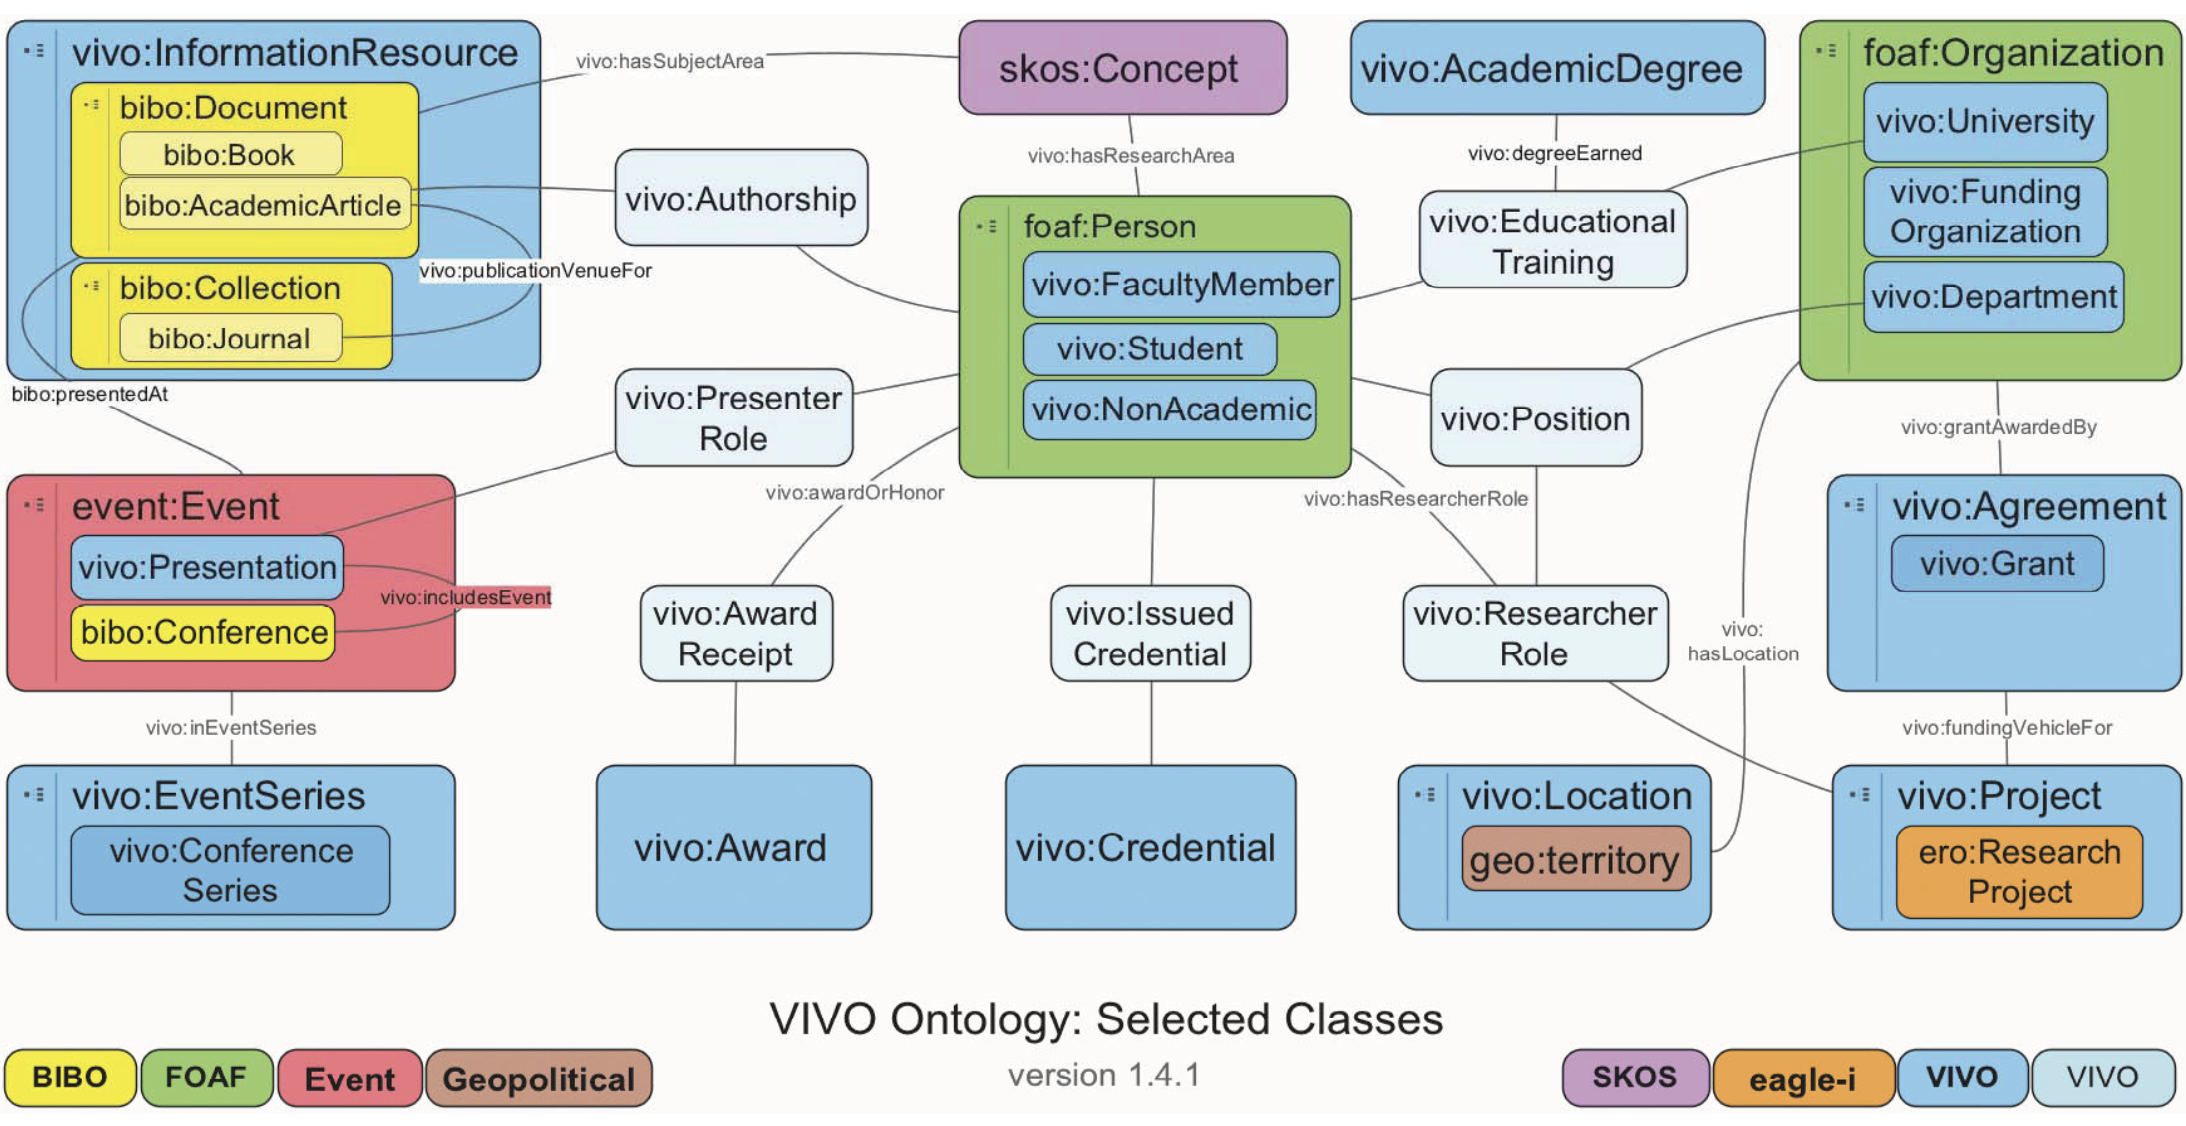
\includegraphics[width=0.8\textwidth]{figures/literature-review/vivo-ontology.png}
     \rule{35em}{0.5pt}
    \caption{Key classes in the VIVO ontology are highlighted alongside their source ontologies, with ``context nodes'' (depicted in light blue) providing temporal details and other information specific to individual relationships. (\textcite{VIVO})}
 \label{fig:vivo-ontology}
\end{figure}

The design of the VIVO Ontology is guided by clear goals, including the ability to represent complex academic relationships and maintain independence from specific implementations to ensure adaptability across diverse institutional contexts.
A hierarchical class structure is employed to define scholarly entities, with an emphasis on modularity and scalability to accommodate the evolving needs of the academic community.
Additionally, the ontology supports the use of external controlled vocabularies and common identifiers to enhance data consistency and interoperability with other systems.

VIVO leverages several well-established ontologies, such as \gls{foaf}, to enrich its representation of scholarly data and ensure interoperability with other systems.
\gls{foaf} is a widely-used ontology designed to describe people, their activities, and their relationships to other people and objects.
The core element of a \gls{foaf} document is the \gls{foaf} vocabulary, which is defined by the namespace: \textless http://xmlns.com/foaf/0.1/\textgreater.
By integrating \gls{foaf}, VIVO can represent entities like researchers and their social networks, enabling a consistent and standard framework for modeling relationships such as collaborations, affiliations, and connections to digital artifacts like websites or profiles.
The primary reason VIVO uses \gls{foaf} is to adopt existing, well-defined vocabularies rather than reinventing the wheel, which promotes interoperability across systems and facilitates data sharing on the Semantic Web.
\gls{foaf}'s compatibility with \gls{lod} principles allows VIVO to easily connect its data with external resources, enhancing discoverability and integration.
For example, \gls{foaf}'s properties such as foaf:Person and foaf:knows align perfectly with VIVO's requirements for describing researchers and their relationships, while maintaining compliance with Semantic Web standards.
By utilizing external ontologies like \gls{foaf}, VIVO not only achieves a more robust and extensible data model but also ensures that its ontology can interact with broader data ecosystems, advancing the goal of creating a globally connected research information infrastructure.
This strategic reuse of established ontologies supports VIVO's vision of openness, interoperability, and scalability in scholarly networking and discovery.
The VIVO Ontology serves as the core of the VIVO application, functioning as a data model and enabling reasoning to infer new relationships based on existing data.
Its flexibility allows institutions to extend the ontology to meet specific local requirements while adhering to its core principles, thereby maintaining compatibility with the broader VIVO ecosystem.
Community-driven efforts play a crucial role in the continuous refinement and expansion of the ontology, ensuring its relevance and alignment with advancements in academic practices.
By supporting the creation of \gls{lod}, the VIVO Ontology facilitates improved research discovery, expert identification, and collaboration across institutions.
%
\section{Large Language Models}\label{sec:large-language-models}
\glspl{llm} have emerged as a transformative innovation in \gls{nlp}, leveraging \gls{dl} techniques to understand, generate, and manipulate human language with unprecedented accuracy.
Fig.~\ref{fig:llms-over-the-years} shows the increasing trend in the number of \glspl{llm} releases and the names of some significant \glspl{llm} proposed from 2019 to 2024.

\begin{figure}[htbp]
    \centering
 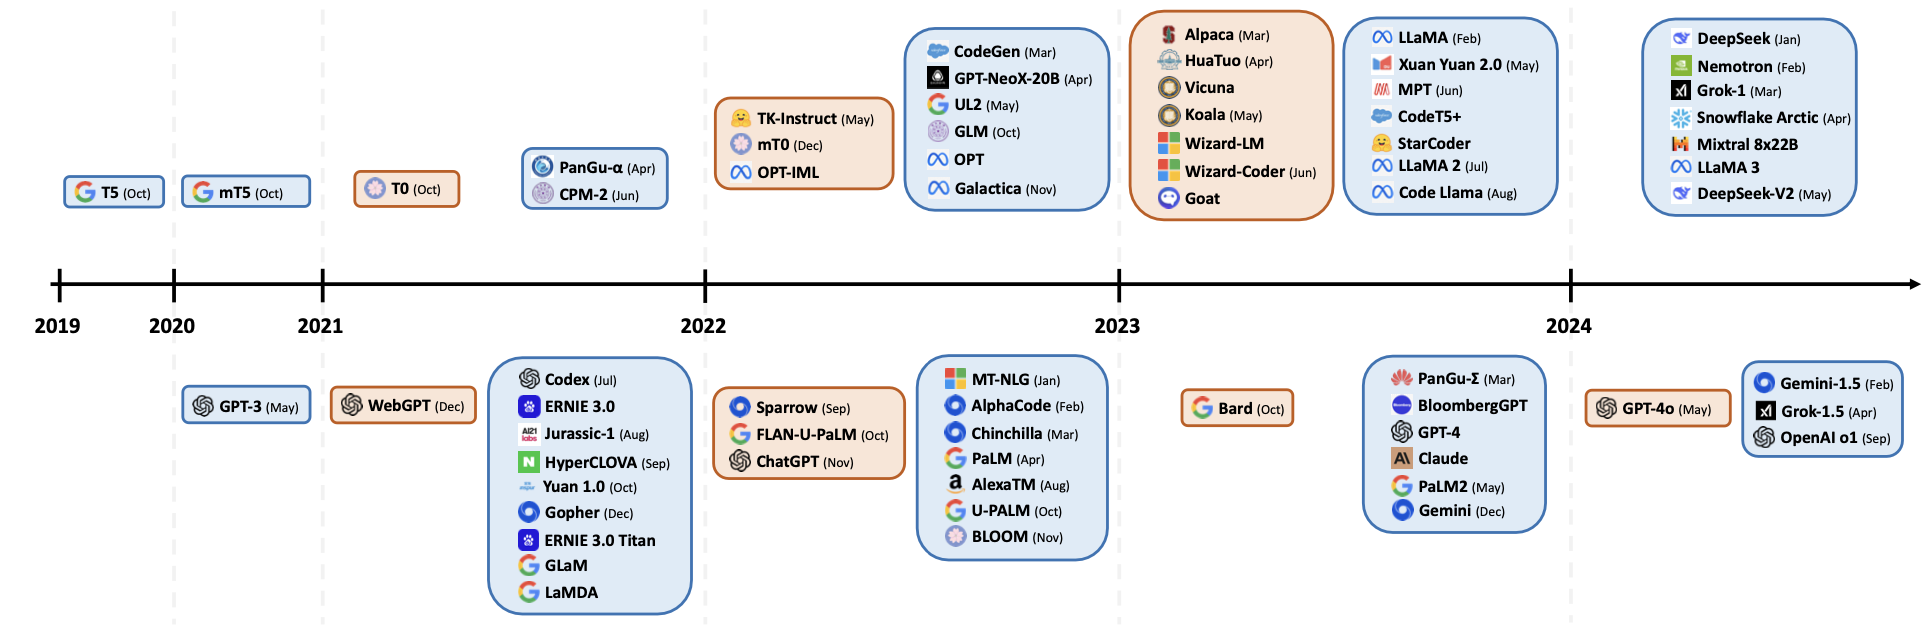
\includegraphics[width=\textwidth]{figures/literature-review/llms-over-the-years.png}
     \rule{35em}{0.5pt}
    \caption{Timeline of \gls{llm} releases: blue cards represent pre-trained models, orange cards denote instruction-tuned models. Open-source models appear on the top, while closed-source models are on the bottom, showing the shift toward open-source and instruction-tuned trends. (\textcite{Naveed2023})}
 \label{fig:llms-over-the-years}
\end{figure}

\glspl{llm}, such as OpenAI's GPT series \cite{Radford2018ImprovingLU}, Google's BERT \cite{Devlin2019BERTPO}, and more recent iterations like GPT-4, are typically built on transformer architectures \cite{Vaswani2017}.
The transformer model introduced a self-attention mechanism that efficiently captures contextual relationships between words across large textual sequences, overcoming limitations of earlier models like \glspl{rnn} and \glspl{lstm} in handling long-range dependencies.
These models are pre-trained on massive corpora containing diverse text from books, articles, and web sources, allowing them to generalize linguistic patterns, syntax, semantics, and even factual knowledge embedded in the data.
According to \textcite{Chang2024}, \glspl{llm} perform a wide range of tasks in \gls{nlp}, often achieving state-of-the-art results across various benchmarks.
Fig.~\ref{fig:llms-overview} provides a broader overview of the organization of \glspl{llm}, categorizing them into seven distinct branches: pre-training, fine-tuning, efficiency, inference, evaluation, applications, and challenges.
These branches reflect the key aspects of the development, deployment, and evaluation of \glspl{llm}.
Pre-training focuses on the foundational step of training models on vast, diverse corpora to learn language representations.
Fine-tuning involves adapting pre-trained models for specific tasks, enhancing their performance on downstream applications.
Efficiency addresses the computational and energy requirements of training and deploying \glspl{llm}, emphasizing methods like parameter-efficient tuning and pruning to reduce resource consumption.
The inference branch examines the process of generating outputs from trained models, focusing on optimizing speed and accuracy.
More advanced capabilities, such as few-shot and zero-shot learning, enable \glspl{llm} to adapt to new tasks with minimal to no task-specific training data, a feature prominently demonstrated by GPT-3 \cite{NEURIPS2020_1457c0d6}.
Evaluation highlights the metrics and benchmarks used to assess \glspl{llm}' performance on various tasks, ensuring they meet quality standards.
Applications span the diverse real-world use cases of \glspl{llm}, from natural language understanding to robotics and multi-modal systems.
Finally, challenges encompass the limitations and issues of \glspl{llm}, including bias, hallucination, and environmental impact, offering directions for future research and improvement.
These branches collectively define the lifecycle and scope of advancements in \glspl{llm} research, providing a comprehensive framework for understanding their capabilities and impact.

\begin{figure}[htbp]
    \centering
 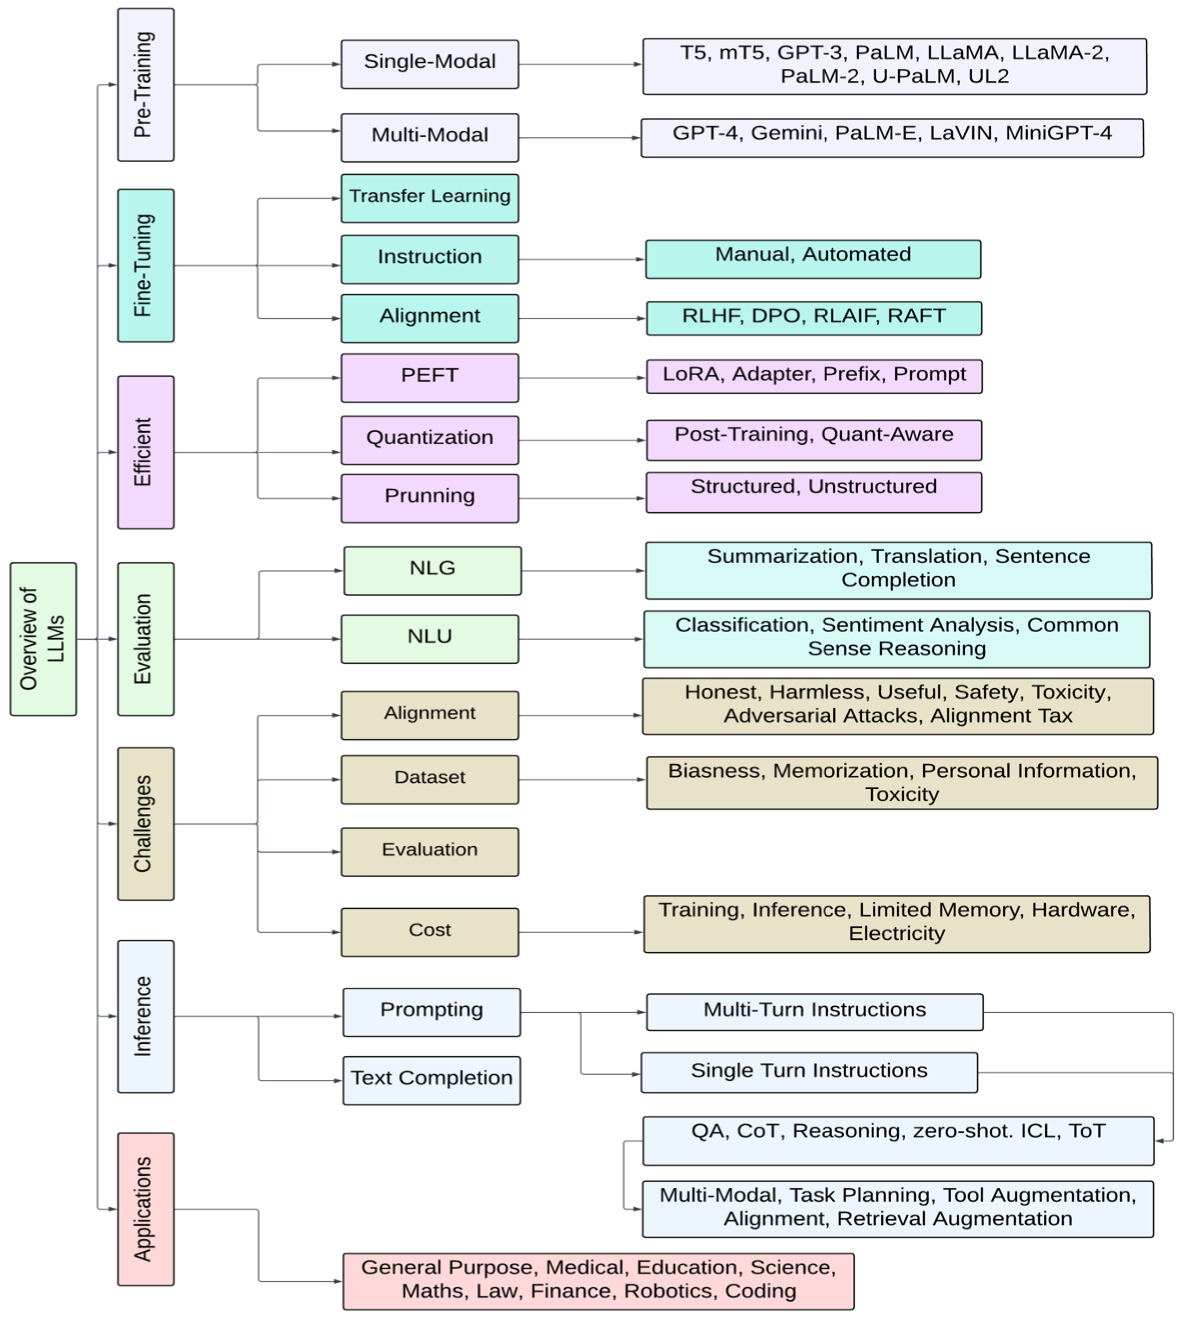
\includegraphics[width=0.8\textwidth]{figures/literature-review/llms-overview.png}
     \rule{35em}{0.5pt}
    \caption{An overview of \glspl{llm} divided into seven branches: pre-training, fine-tuning, efficiency, evaluation, challenges, inference, and applications. (\textcite{Naveed2023})}
 \label{fig:llms-overview}
\end{figure}

This adaptability has made \glspl{llm} suitable for tasks requiring contextual reasoning, dialogue systems, and even code generation, as seen in models like Codex \cite{Chen2021EvaluatingLL}, which powers tools such as GitHub Copilot\footnote{\url{https://github.com/features/copilot}}.
The applications of \glspl{llm} span numerous domains, reflecting their versatility and broad impact.
In industry, \glspl{llm} power conversational agents, customer service bots, and content creation tools.
In research and education, they facilitate automated summarization of scientific literature, personalized tutoring, and question-answering systems to support knowledge discovery.
The integration of \glspl{llm} with domain-specific knowledge graphs and ontologies further enhances their reliability, particularly in specialized areas such as medicine, law, and scientific discovery \cite{Yang2024}.
Despite their strengths, \glspl{llm} have some limitations.
One important problem is their dependence on vast computational resources for training, which has implications for environmental sustainability \cite{Strubell2019EnergyAP}.
Furthermore, \glspl{llm} tend to propagate biases present in the training data, leading to inconsistencies when deployed in real-world applications \cite{Naveed2023}.
They also suffer from factual inaccuracies and hallucinations, where the model generates plausible yet incorrect information \cite{Chang2024}, which limits their applicability in high-stakes environments requiring factual precision.
Moreover, the lack of interpretability in \glspl{llm} remains a significant challenge, as their outputs are generated from complex internal representations that are not easily explainable, leading to questions about trust and accountability \cite{Naveed2023}.
Nevertheless, the advantages of \glspl{llm} are substantial, as they offer unprecedented performance in language-related tasks, significant generalizability, and the ability to operate across diverse applications without extensive task-specific engineering.
In their study, \textcite{Naveed2023} discuss that current research about \glspl{llm} efforts are focused on addressing their limitations, particularly improving energy efficiency, reducing bias, enhancing factual accuracy, and developing methods for better interpretability.
As \glspl{llm} continue to evolve, their integration with structured knowledge systems and advancements in alignment with human intent are likely to redefine their role in solving complex problems across industries.
%
\section{Retrieval-Augmented Generation}\label{sec:retrieval-augmented-generation}
\acrfull{rag} improves \glspl{llm} by integrating real-time data retrieval into the generative process \cite{singh2025}.
Unlike static \glspl{llm} that rely on pre-trained knowledge, \gls{rag} dynamically retrieves relevant external information, improving response accuracy, contextual relevance and updateability \cite{Fan2024, singh2025}.

\begin{figure}[htbp]
  \centering
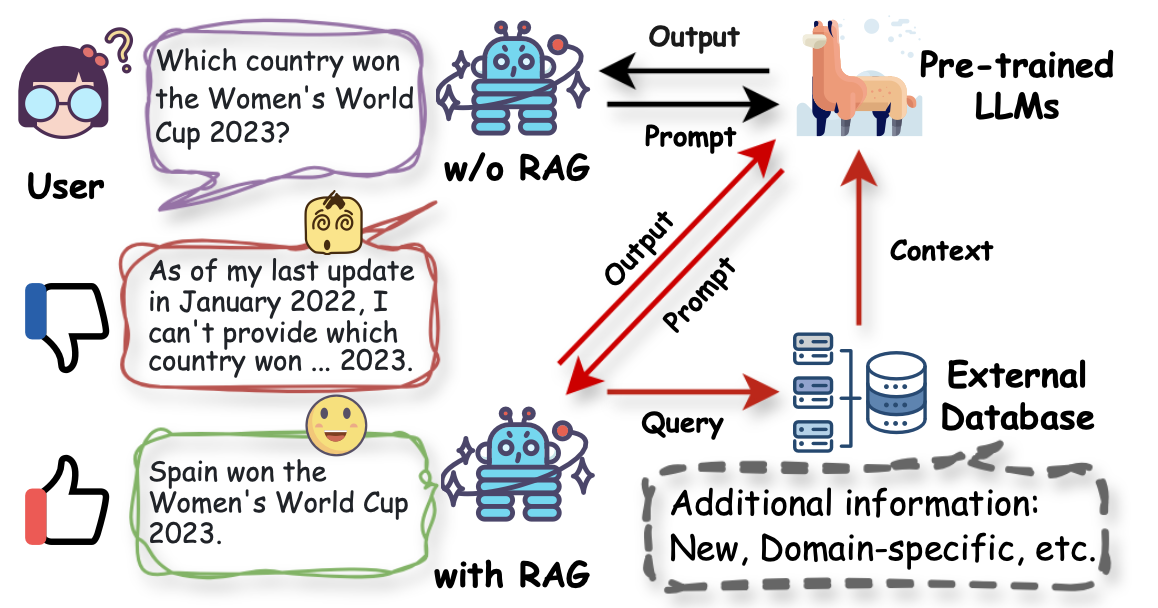
\includegraphics[width=.7\textwidth]{figures/literature-review/rag-no-rag-example.png}
   \rule{35em}{0.5pt}
  \caption{An example of the limitations of \glspl{llm} without retrieval mechanisms (top) and the benefits of \gls{rag} with real-time data retrieval (bottom) (\textcite{Fan2024})}
\label{fig:rag-no-rag-example}
\end{figure}

When a user's query requires information beyond the training data of a \gls{llm}, such as real-time knowledge or unseen facts, the model's response may be outdated or incomplete.
In such cases, standard \glspl{llm} without external retrieval mechanisms struggle to provide accurate answers, as illustrated in the upper part of the Fig.~\ref{fig:rag-no-rag-example}.
Here, the model fails to answer a simple fact-based question about the winner of the 2023 Women's World Cup due to its training data cutoff.
However, with \gls{rag}, as shown in the lower part of the image, the system retrieves relevant information from an external database before generating a response.
This enables the model to produce up-to-date and contextually accurate answers by grounding its output in real-world knowledge.
Fig.~\ref{fig:rag-components} shows the three main components of \gls{rag}:
\begin{itemize}
    \item \textbf{Retrieval}: queries external sources such as knowledge bases, APIs or vector databases, using dense vector search and advanced transformer-based models to improve accuracy.
    \item \textbf{Augmentation}: processes, extracts and synthesises the retrieved data to align it with the user's query.
    \item \textbf{Generation}: combines the retrieved information with the \gls{llm}'s internal knowledge to produce coherent and contextually relevant answers. 
\end{itemize}
	
\begin{figure}[htbp]
    \centering
 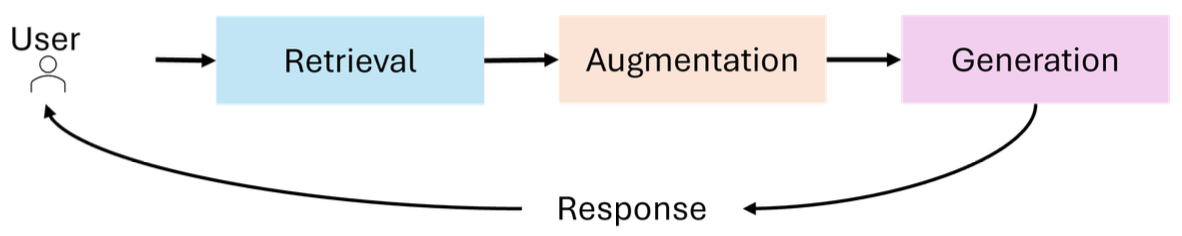
\includegraphics[width=.65\textwidth]{figures/literature-review/RAGcomponents.png}
     \rule{35em}{0.5pt}
    \caption{\gls{rag} components (\textcite{singh2025})}
 \label{fig:rag-components}
\end{figure}

The evolution of \gls{rag} has given rise to several paradigms, each of which refines the interaction between retrieval and generation to improve contextual accuracy, scalability and reasoning capabilities.
From the basic Na\"ive \gls{rag} to the more sophisticated Advanced \gls{rag}, Modular \gls{rag} and Graph\gls{rag}, these approaches have progressively addressed major limitations.
The newest and most powerful paradigm, Agentic \gls{rag}, introduces autonomous agents that dynamically adapt retrieval strategies, optimise workflows and enable complex multi-stage reasoning.
Each paradigm is briefly described in the next subsections.
Table~\ref{table:rag-paradigms-comparison} provides a comparison of the key features, strengths and challenges of these \gls{rag} paradigms.

\subsection*{Na\"ive \gls{rag}}\label{sec:naive-rag}
Na\"ive \gls{rag} is the most fundamental implementation of \gls{rag}, characterized by a straightforward retrieve-read framework \cite{gao_retrieval-augmented_2024}.
It consists of three main steps: indexing, retrieval, and generation \cite{gao_retrieval-augmented_2024,singh2025}.
During indexing, raw data from various sources (e.g., PDFs, Word documents, HTML) is cleaned, segmented into smaller text chunks, and embedded into a vector representation using an embedding model before being stored in a vector database.
When a user poses a query, the system retrieves the most relevant text chunks based on semantic similarity using the same embedding model.
These retrieved chunks are then incorporated into the generation phase, where a \gls{llm} synthesizes a response using both the retrieved information and its internal knowledge.
While Na\"ive \gls{rag} effectively enhances \glspl{llm} by integrating external knowledge, it suffers from several limitations, described as follows.
Retrieval inefficiencies: the retrieved chunks may be irrelevant, misaligned, or miss crucial context, reducing the quality of responses \cite{gao_retrieval-augmented_2024,singh2025}.
Hallucinations: the \gls{llm} may generate content unsupported by retrieved data, leading to factual inaccuracies \cite{gao_retrieval-augmented_2024}.
Redundancy and inconsistency: retrieved information may be overlapping or disjointed, making it challenging to generate coherent answers \cite{gao_retrieval-augmented_2024}.
Limited adaptability: a single retrieval pass based on the original query might not capture sufficient context, restricting performance in complex tasks \cite{gao_retrieval-augmented_2024,singh2025}.
Despite its simplicity, Na\"ive \gls{rag} provided the foundation for more advanced \gls{rag} paradigms, such as Advanced \gls{rag} and Modular \gls{rag}, which introduce retrieval optimization, re-ranking mechanisms, and multi-step reasoning to address these challenges.

\subsection*{Advanced \gls{rag}}\label{sec:advanced-rag}
Advanced \gls{rag} enhances the limitations of Na\"ive \gls{rag} by integrating sophisticated retrieval optimization techniques and semantic understanding to improve information retrieval and generation quality \cite{gao_retrieval-augmented_2024}.
Unlike Na\"ive \gls{rag}, which relies on simple keyword-based retrieval, Advanced \gls{rag} employs \gls{dpr} \cite{Karpukhin2020} and neural ranking algorithms to prioritize relevant information \cite{singh2025}.
It introduces pre-retrieval optimizations such as query expansion, metadata enrichment, and indexing improvements to refine the quality of retrieved data.
Additionally, it implements post-retrieval techniques like context re-ranking, summarization, and adaptive filtering, ensuring that the retrieved information aligns more effectively with the user query before being fed into the language model.
Furthermore, Advanced \gls{rag} supports multi-hop retrieval, allowing the system to retrieve and combine insights from multiple sources to generate well-informed and contextually aware responses.
These enhancements make it more scalable and precise, making it well-suited for knowledge-intensive applications such as scientific research, legal reasoning, and enterprise search solutions.
However, it comes with challenges such as higher computational overhead and latency due to complex retrieval and ranking processes.

\subsection*{Modular \gls{rag}}\label{sec:modular-rag}
Modular \gls{rag} addresses the limitations of Na\"ive and Advanced \gls{rag} by incorporating flexible and composable components, enabling greater adaptability and optimization for specific use cases \cite{gao_retrieval-augmented_2024}.
In contrast to the linear pipeline of traditional \gls{rag}, Modular \gls{rag} enables independent modification and replacement of retrieval, augmentation, and generation modules, making it highly customizable.
According to \cite{singh2025}, key enhancements include hybrid retrieval strategies, where both sparse (e.g., BM25) and dense retrieval \cite{Karpukhin2020} (e.g., \gls{dpr}) techniques are combined for better query matching, and multi-source retrieval, which integrates structured (databases, \glspl{kg}) and unstructured (documents, APIs) sources.
Moreover, modular \gls{rag} introduces new modules like adaptive search, memory, and task-specific adapters, along with new patterns such as iterative retrieval and dynamic module reconfiguration, enhancing flexibility and precision across diverse applications \cite{gao_retrieval-augmented_2024}.
It also supports dynamic query rewriting and multi-step reasoning, allowing iterative refinements to retrieval results.
Its modular design makes it ideal for domain-specific tasks, such as financial analytics and scientific research, where different retrieval and augmentation techniques are needed.
However, this paradigm faces challenges in complex data integration, requiring handling of unstructured, semi-structured, and structured data; system orchestration, demanding precise workflow management across modular components; and component selection and optimization, ensuring individual modules are fine-tuned and effectively integrated for optimal performance.
Fig.~\ref{fig:naive-advanced-modular-rag} illustrates the three \gls{rag} paradigms just described, Na\"ive, Advanced and Modular \gls{rag}, highlighting their key components, optimisations and structural differences.
\begin{figure}[htbp]
    \centering
 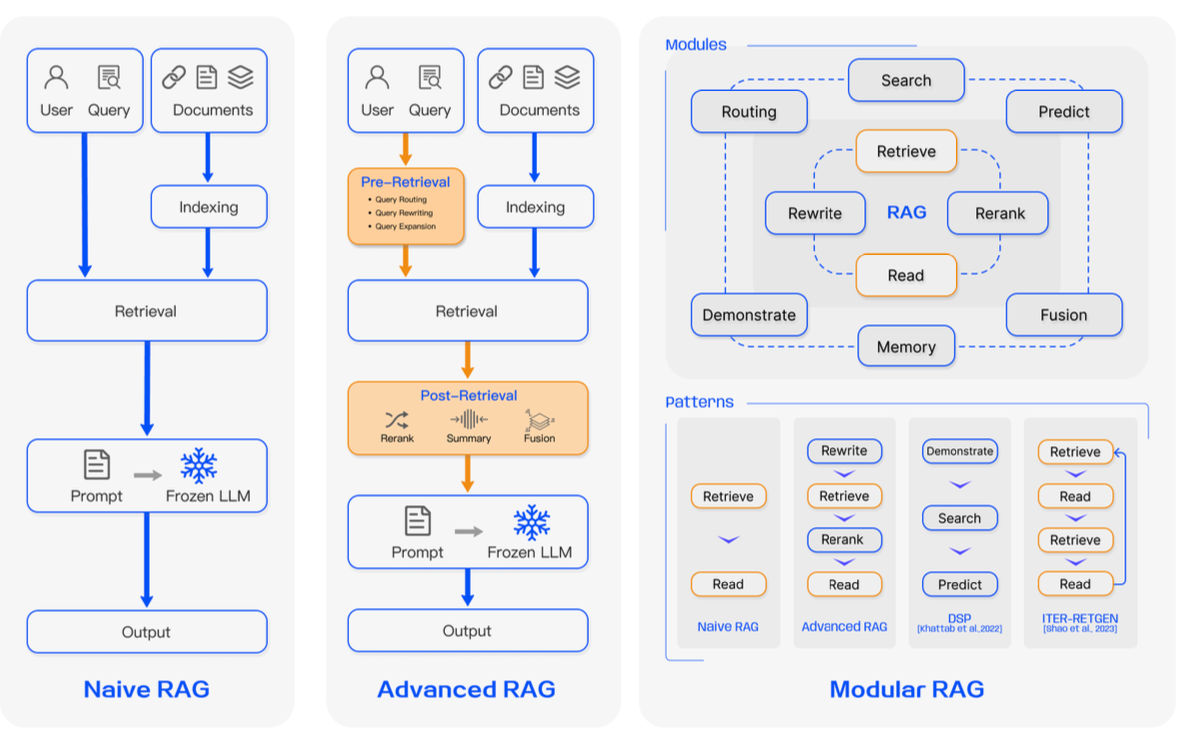
\includegraphics[width=.75\textwidth]{figures/literature-review/naive-advanced-modular-rag.png}
     \rule{35em}{0.5pt}
    \caption{Na\"ive, Advanced and Modular \gls{rag} architectures (\textcite{gao_retrieval-augmented_2024})}
 \label{fig:naive-advanced-modular-rag}
\end{figure}

\subsection*{Graph\gls{rag}}\label{sec:graph-rag}
Graph\gls{rag} is an advanced \gls{rag} framework that leverages structured \glspl{kg}, as illustrated in Fig.~\ref{fig:graph-rag-architecture} , to improve contextual understanding and response generation by \glspl{llm} \cite{peng2024graphragsurvey,singh2025}.
Unlike traditional \gls{rag} approaches that rely solely on retrieving textual information, Graph\gls{rag} incorporates relational knowledge by retrieving structured graph elements, such as nodes, triples, paths, or subgraphs, from a pre-constructed graph database.
This allows for more accurate and context-aware responses, as it captures entity relationships that text-based methods often overlook \cite{singh2025}.
One of the key distinctions between Graph\gls{rag} and standard \gls{rag} is its ability to maintain and utilize explicit structural connections, whereas text-based \gls{rag} primarily depends on similarity-based retrieval from unstructured text corpora.
Graph\gls{rag} thus reduces redundancy and enhances global information retrieval by abstracting and summarizing textual data into a more structured form.
Among its advantages, Graph\gls{rag} enables more precise and comprehensive retrieval, effectively capturing relational knowledge that improves factual consistency and mitigates hallucination.
Additionally, it facilitates query-focused summarization by retrieving subgraphs that include broader contextual information, reducing verbosity in responses.
However, Graph\gls{rag} also presents limitations, including scalability challenges due to the exponential growth of subgraph candidates and the dependency on high-quality, well-structured graph data \cite{singh2025}.
Integrating graph-based retrieval with unstructured retrieval mechanisms adds complexity to implementation, making Graph\gls{rag} more computationally demanding than traditional \gls{rag} approaches \cite{peng2024graphragsurvey,singh2025}.

\begin{figure}[htbp]
    \centering
 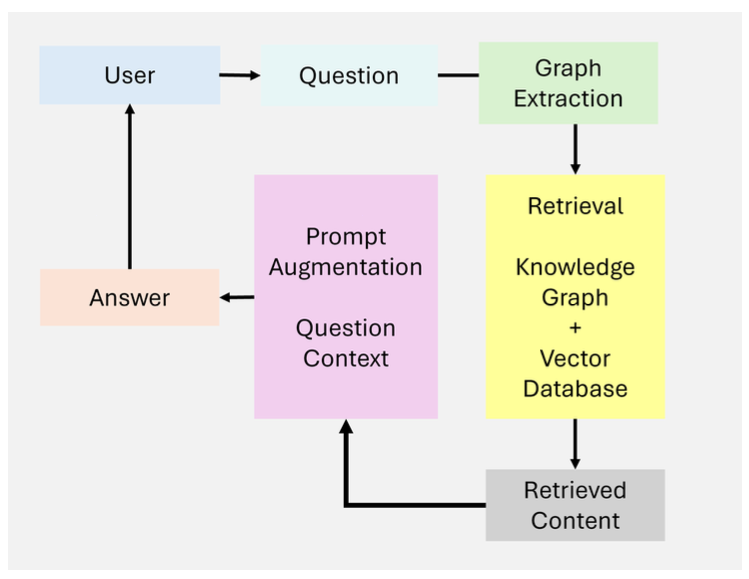
\includegraphics[width=.65\textwidth]{figures/literature-review/graphRAG.png}
     \rule{35em}{0.5pt}
    \caption{Graph\gls{rag} architecture (\textcite{singh2025})}
 \label{fig:graph-rag-architecture}
\end{figure}

\subsection*{Agentic \gls{rag}}\label{sec:agentic-rag}
Agentic\gls{rag} extends traditional \gls{rag} frameworks by integrating autonomous agents that dynamically manage retrieval, reasoning, and response generation workflows \cite{singh2025}.
Unlike standard \gls{rag} systems, which rely on predefined retrieval pipelines, Agentic\gls{rag} incorporates agentic design patterns such as reflection, planning, tool use, and multi-agent collaboration to enable adaptive decision-making and iterative refinement.
These autonomous agents assess query complexity, refine search strategies, and optimize knowledge integration, leading to improved contextual accuracy and scalability.
A key advantage of Agentic\gls{rag} is its ability to manage multi-step reasoning processes, allowing for more precise responses to complex queries.
By dynamically orchestrating workflows, these systems enhance retrieval efficiency and minimize hallucinations by iteratively validating retrieved content.
However, the increased complexity of Agentic\gls{rag} poses challenges, including higher computational overhead and the need for sophisticated coordination mechanisms among multiple agents.
An example of a Multi-Agent Agentic\gls{rag} architecture is shown in Fig.~\ref{fig:multi-agent-agentic-rag}.
Additionally, while it improves adaptability, the unpredictability of agent-driven workflows can introduce variability in response generation.
Despite these challenges, Agentic\gls{rag} is particularly well-suited for domains requiring dynamic adaptability, such as financial analytics, healthcare diagnostics, and legal research, where multi-agent collaboration and iterative refinement enhance the reliability of \gls{ai}-generated insights \cite{singh2025}.

\begin{figure}[htbp]
    \centering
 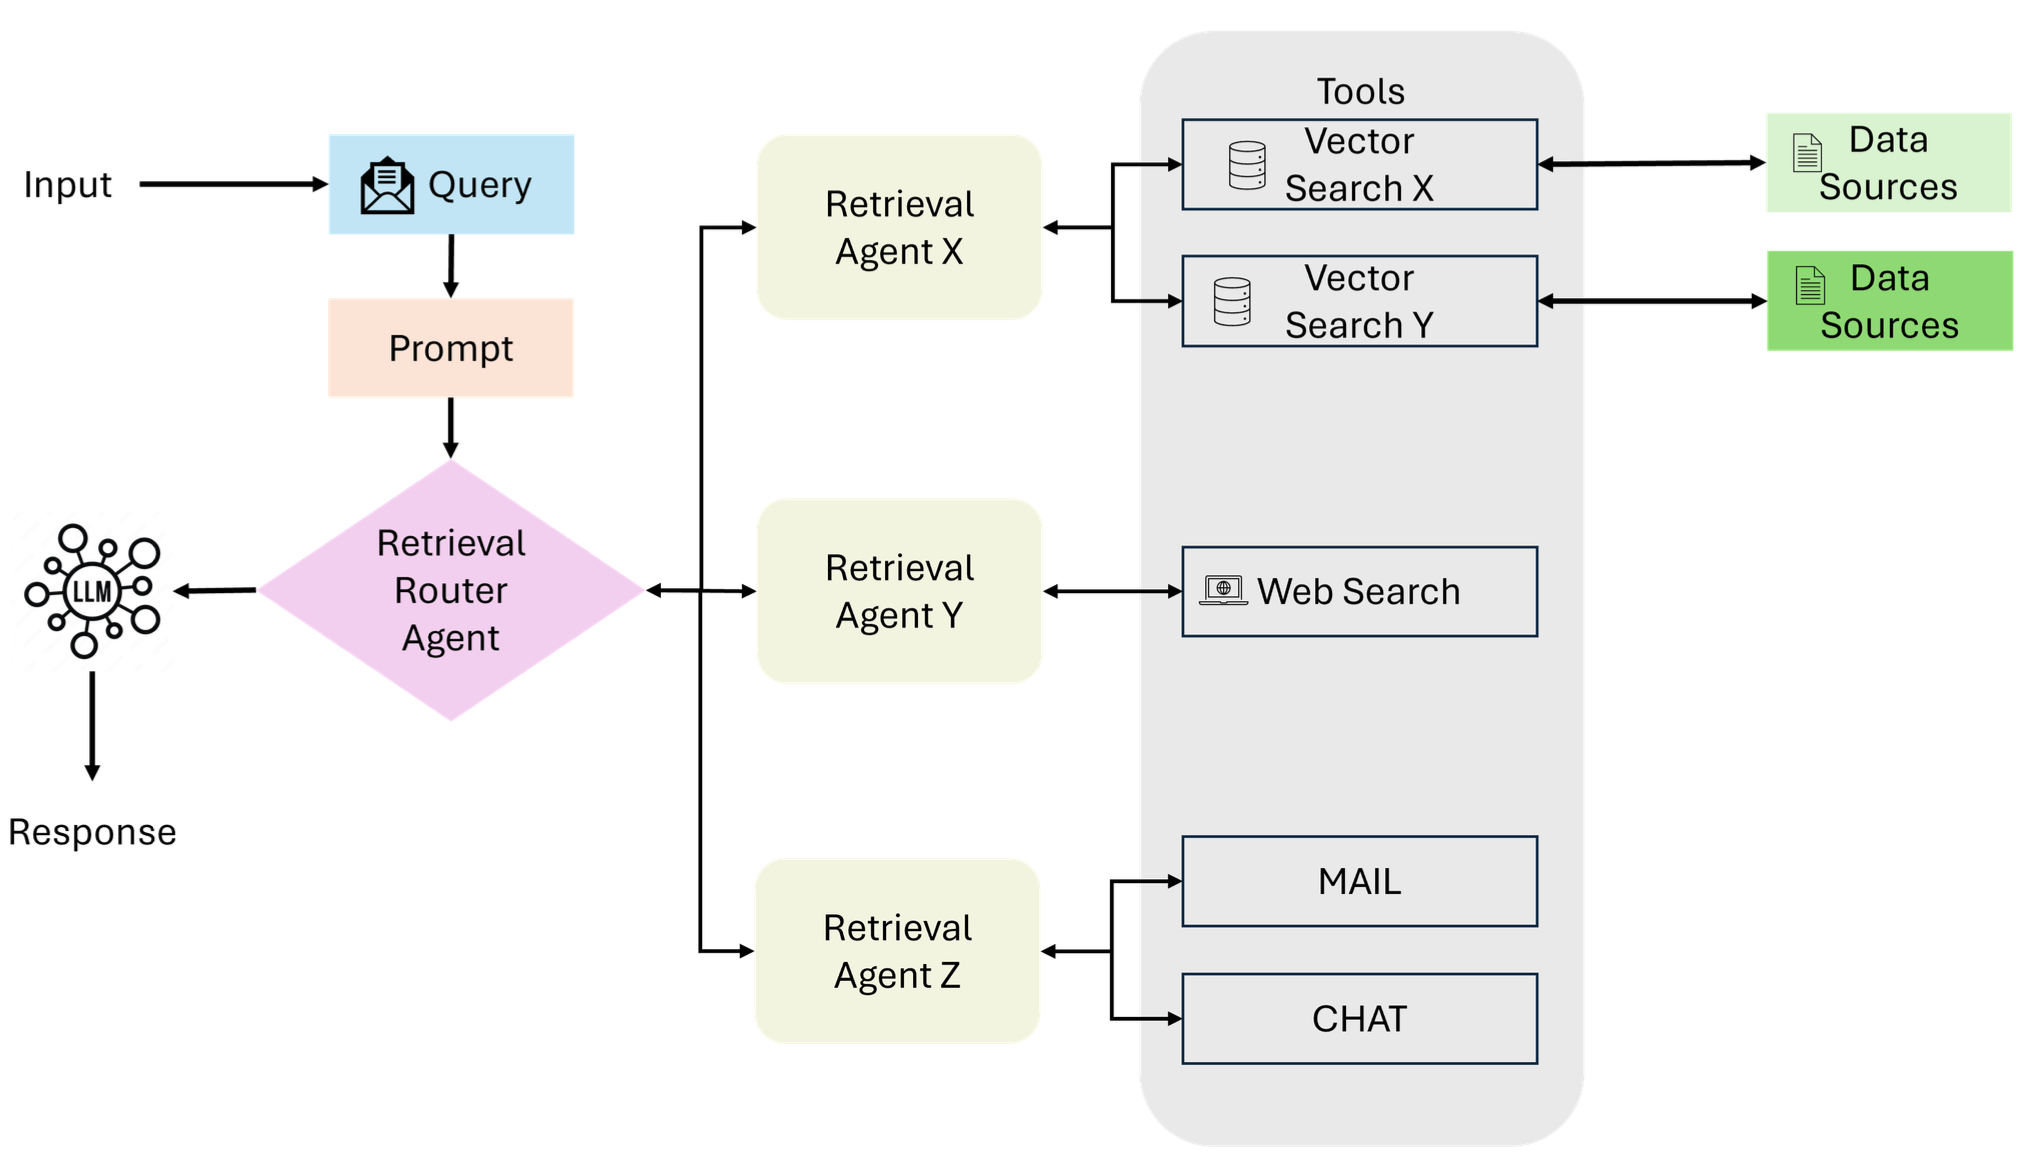
\includegraphics[width=.8\textwidth]{figures/literature-review/multi-agent-agentic-rag.png}
     \rule{35em}{0.5pt}
    \caption{Multi-Agent Agentic\gls{rag} architecture (\textcite{singh2025})}
 \label{fig:multi-agent-agentic-rag}
\end{figure}

\begin{table}[htbp]
    \centering
    \scriptsize
    \begin{tabularx}{\textwidth}{|>{\centering\arraybackslash}p{1.5cm}|X|X|X|}
      \hline
      \textbf{\gls{rag} Paradigm} & \textbf{Key Features} & \textbf{Strengths} & \textbf{Challenges}\\
      \hline
          \begin{center}
            Na\"ive
          \end{center} & \begin{itemize}[nosep, left=0pt]
        \item Keyword-based retrieval (e.g., TF-IDF, BM25)
      \end{itemize} & \begin{itemize}[nosep, left=0pt]
        \item Simple and easy to implement
        \item Suitable for fact-based queries
      \end{itemize}& \begin{itemize}[nosep, left=0pt]
        \item Retrieval inefficiency
        \item Hallucinations
        \item Redundancy and inconsistency
        \item Limited adaptability
      \end{itemize}\\
      \hline
      \begin{center}
      Advanced
      \end{center} & \begin{itemize}[nosep, left=0pt]
        \item Dense retrieval models (e.g., DPR)
        \item Neural ranking and re-ranking
        \item Multi-hop retrieval
      \end{itemize} & \begin{itemize}[nosep, left=0pt]
        \item High precision retrieval
        \item Improved contextual relevance
      \end{itemize} & \begin{itemize}[nosep, left=0pt]
        \item Higher computational overhead
        \item Latency
      \end{itemize}\\
      \hline
      \begin{center}
        Modular
      \end{center} & \begin{itemize}[nosep, left=0pt]
        \item Hybrid retrieval (sparse and dense)
        \item Tool and API integration
        \item Composable, domain-specific pipelines
      \end{itemize} & \begin{itemize}[nosep, left=0pt]
        \item High flexibility and customization
        \item Suitable for diverse applications
        \item Scalable
      \end{itemize} & \begin{itemize}[nosep, left=0pt]
        \item Complex data integration
        \item System orchestration and workflow management
        \item Component selection and optimization
        \item Maintenance
      \end{itemize}\\
      \hline
      \begin{center}
        Graph
      \end{center} & \begin{itemize}[nosep, left=0pt]
        \item Integration of graph-based structures
        \item Multi-hop reasoning
        \item Contextual enrichment via nodes
      \end{itemize}& \begin{itemize}[nosep, left=0pt]
        \item Relational reasoning capabilities
        \item Mitigates hallucinations
        \item Ideal for structured data tasks
      \end{itemize}& \begin{itemize}[nosep, left=0pt]
        \item Scalability challenges
        \item Dependency on high-quality graph data
        \item Complexity of integration
      \end{itemize}\\
      \hline
      \begin{center}
        Agentic
      \end{center} & \begin{itemize}[nosep, left=0pt]
        \item Autonomous agents
        \item Dynamic decision-making
        \item Iterative refinement and workflow optimization
      \end{itemize}& \begin{itemize}[nosep, left=0pt]
        \item Adaptable to real-time changes
        \item Scalable for multi-domain tasks
        \item High accuracy
      \end{itemize} & \begin{itemize}[nosep, left=0pt]
        \item Coordination complexity
        \item Computational overhead
        \item Scalability challenges
      \end{itemize}\\
      \hline
    \end{tabularx}
    \caption{\gls{rag} paradigms comparison adapted from \textcite{singh2025} and extended by the author}
    \label{table:rag-paradigms-comparison}
  \end{table}
%
\section{Recommender Systems}\label{sec:recommender-systems}
The task of recommender systems is to use users' data and their current and historical preferences with the goal of making predictions about users' possible future likes and interests \cite{Lu2012}.

In recommender systems, \gls{ml} models are used to predict the rating $r_{ui}$ of a user $u$ on an item $i$.
At inference time, the system recommends to each user $u$ the items $I$ having highest predicted rating $r_{ui}$.
It is therefore necessary to collect user feedback, so that we can have a ground truth for training and evaluating our models.
Explicit Feedback is a rating explicitly given by the user to express their satisfaction with an item.
Implicit Feedback assumes that user-item interactions are an indication of preferences.

The two main approaches in recommender systems are \gls{cbf} and \gls{cf}, often combined in hybrid methods \cite{Ko2022}.

\gls{cbf} is a method for recommending articles with attributes similar to those that users like and recommends them based on article information \cite{Vallet2006}.
According to \textcite{salter2006cinemascreen}, such filtering has a major drawback: it recommends only data on articles that are closely related to data on articles that a user has considered in the past. Because of this, the system struggles to recommend new articles. 

\gls{cf} relies on user-item interactions, such as ratings or clicks, to identify patterns and recommend items that were liked by similar users.
It is effective, but suffers from 3 problems such as: the sparsity problem, that occurs when there is not enough data available for recommendation \cite{Plexousakis2005}.
Another important problem is the cold start problem, which occurs when there is no evaluation data, that is, when a new user enters the system \cite{WEI201729}.
Finally, gray sheep is a problem in which there is only a small number of users with similar evaluation data to that of the individual user, and thus there are difficulties in providing recommendations \cite{Gras2016}.

Hybrid filtering systems integrate multiple recommendation techniques, such as \gls{cbf} and \gls{cf}, to address the shortcomings of each method and improve overall recommendation quality \cite{Ko2022}.
By combining these approaches, hybrid systems can utilize both item attributes and user behavior to create a more comprehensive understanding of preferences.
This combination enhances recommendation accuracy, increases diversity, and provides a more robust solution adaptable to various scenarios, making hybrid systems a superior choice for personalized recommendations.

\subsection*{Recommender Systems in Research Field}\label{sec:recommender-systems-in-research-field}
Most of the existing works of recommender systems in the literature regarding the field of research are based on suggesting research papers, or academic collaborators.
The following describes the work found during the literature review regarding these systems.

\textcite{refore} proposed the REFORE system, a hybrid recommender system specifically designed to assist researchers in managing information overload by providing high-quality and personalized recommendations of research papers.
The system integrates bibliometric measures, such as journal impact factors and author H-indexes, into its recommendation process, thereby emphasizing the quality of both the items (papers) and the users (researchers) involved.
REFORE employs a \gls{cbf} approach to match user preferences with paper content, using metadata such as keywords, abstracts, and citations.
It represents papers as vectors in a linguistic framework, assigning importance scores to keywords, which are then matched to user profiles.
The structure of the system is shown in Fig.~\ref{fig:refore}.
These profiles are built dynamically based on the researcher's past publications and manually input preferences.
Additionally, a \gls{cf} mechanism is implemented to leverage the feedback and preferences of similar users, identifying relevant items based on shared interests.
The system adopts a two-phase feedback process: users can evaluate recommendations as relevant or irrelevant and later provide qualitative assessments of the papers they read.
This feedback not only improves future recommendations but also helps refine the underlying quality measures for papers and authors.
A key innovation in REFORE is its re-ranking process, which combines \gls{cbf} and \gls{cf} outputs with quality scores derived from bibliometric data.
Papers are ranked not only by their relevance to the user but also by their scientific quality and novelty.
To handle the fuzziness inherent in user preferences and item quality, REFORE utilizes a fuzzy linguistic modeling approach, which ensures flexibility and granularity in assessing and aggregating preferences.
This linguistic framework allows for precise and interpretable measurements of similarities and quality across items and users.

\begin{figure}[htbp]
    \centering
 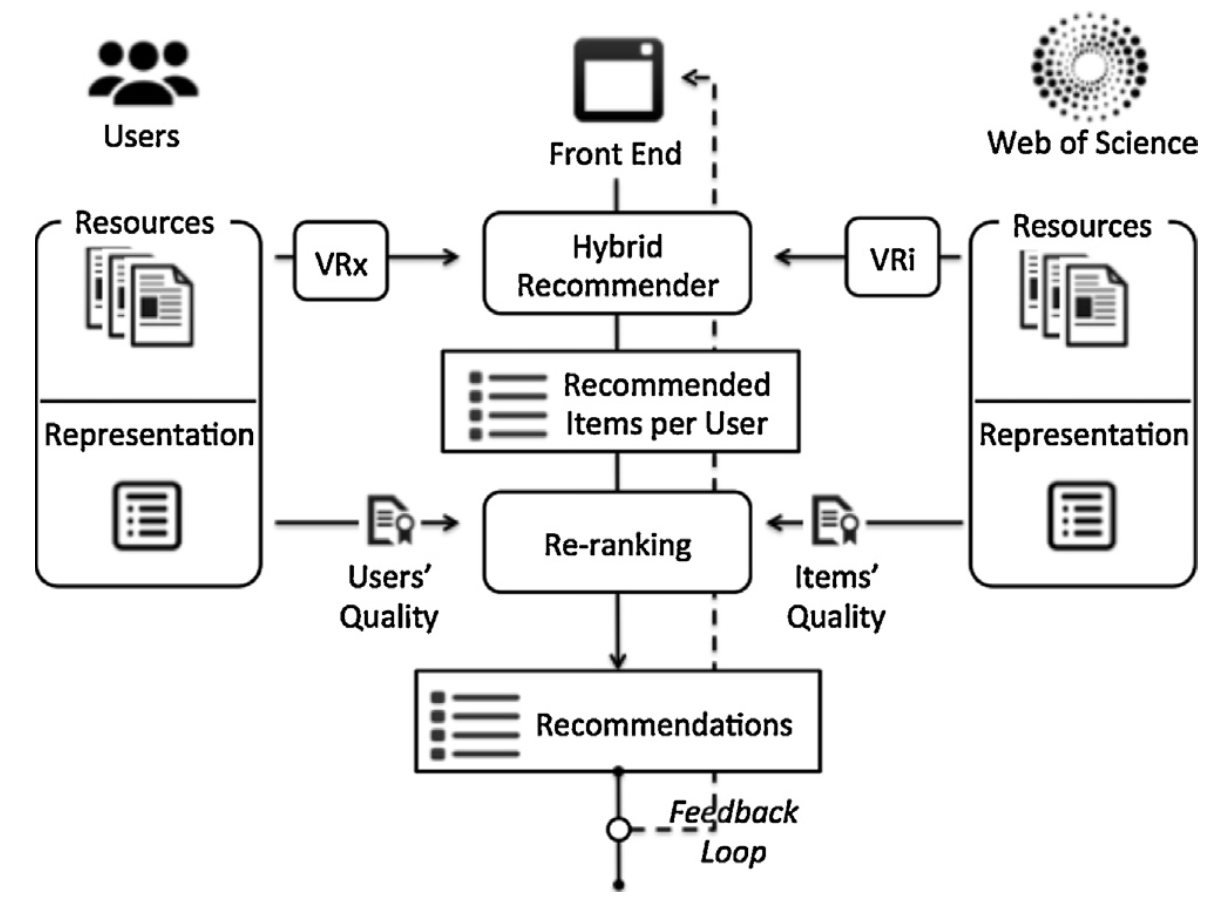
\includegraphics[width=0.6\textwidth]{figures/literature-review/refore.png}
     \rule{35em}{0.5pt}
    \caption{Structure of REFORE system (\textcite{refore})}
 \label{fig:refore}
\end{figure}

In terms of evaluation, the system was tested with a group of researchers from multiple institutions over a year-long period.
Researchers received monthly recommendations based on newly published papers from the Web of Science database, and their feedback was collected to measure the system's effectiveness.
The experimental results demonstrated the system's ability to deliver high-quality and personalized recommendations, outperforming traditional methods by incorporating bibliometric quality measures and user feedback into the hybrid recommendation strategy.

\textcite{Kanwal2024} proposed a research paper recommendation system, integrating citation networks and collaboration networks to provide high-quality and relevant suggestions to researchers.
This approach, named \gls{rrmf}, addresses challenges such as the cold-start problem, data sparsity, and semantic ambiguity.
The proposed methodology involves generating a multi-level citation network, where the focal paper of interest (PI) serves as the central node.
Citation relationships are explored up to six levels, leveraging both forward (citing) and backward (cited by) links.
To evaluate the relevance of papers within the network, bibliographic coupling and co-citation strengths are computed, quantifying the similarity of papers based on shared citations or references.
A candidate score is derived for each paper, which is used to filter irrelevant documents and focus on those most closely related to the paper of interest.
Additionally, centrality measures (such as betweenness, degree, closeness, and eigenvector centrality) are applied to rank papers based on their structural significance within the network.
Papers with high centrality scores are selected for further analysis.
The system extends beyond citation networks by incorporating collaboration networks of authors.
Authors are extracted from top-ranked papers, and their collaboration networks are analyzed using centrality and social measures to identify influential researchers.
These author-based insights contribute to refining paper recommendations, ensuring that suggested papers come from prominent authors within the field.
To evaluate the system, the AMiner dataset, comprising nearly 4.8 million papers and over 45 million citation relationships, was used.
The system's performance was benchmarked using metrics such as \gls{map}, \gls{mrr}, and \gls{ndcg}.
Experimental results demonstrated that the \gls{rrmf} outperformed traditional systems, such as Google Scholar and previous citation-based methods, by achieving higher precision and recall.
The incorporation of multi-level citation analysis and author collaboration measures significantly improved the quality and relevance of recommendations.

\textcite{Murali2019} proposed a research paper recommender system using a user-based \gls{cf} approach.
The goal of the system is to recommend research papers tailored to a user's interests by analyzing their preferences and similarities with other users.
The authors addressed the challenge of information overload faced by researchers due to the rapid growth in the number of research publications.
The system operates by collecting a dataset of user-paper interactions, which includes attributes such as user IDs, paper IDs, and ratings assigned by users to the papers. Based on this data, the system calculates the similarity between users using the cosine similarity measure. This approach evaluates the resemblance between user profiles by treating their preferences as vectors and computing the cosine of the angle between them.
Users with similar interests are identified, and recommendations are generated by predicting ratings for papers based on the ratings given by these similar users.
The block diagram of the system architecture is shown in Fig.~\ref{fig:murali}.
To improve the quality of recommendations, the system utilizes a prediction rating mechanism, which assigns a predicted score to papers based on the \gls{cf} model.
Papers with higher predicted ratings are recommended to the user, ensuring that suggestions align with their preferences.
The authors also implemented a ``user-link formation'' step to construct the \gls{cf} model, leveraging the collective behavior of similar users to refine recommendations further.

\begin{figure}[htbp]
    \centering
 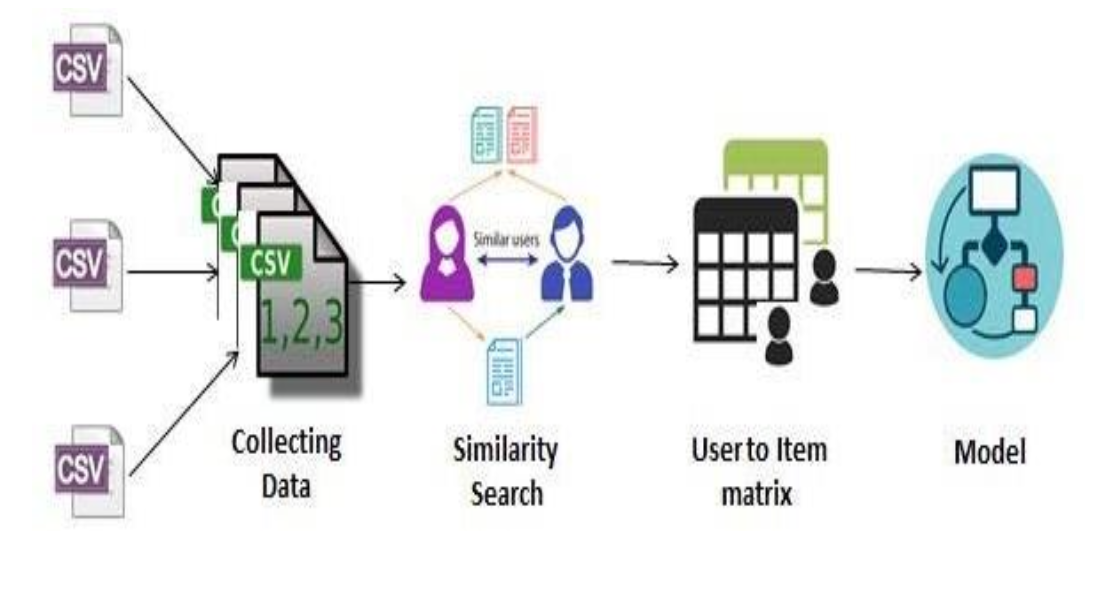
\includegraphics[width=0.65\textwidth]{figures/literature-review/murali.png}
     \rule{35em}{0.5pt}
    \caption{Block diagram of the system architecture (\textcite{Murali2019})}
 \label{fig:murali}
\end{figure}

For evaluation, the system was tested on a dataset comprising 135 users and their interactions with research papers.
Performance was measured using metrics like \gls{mae} and \gls{rmse} to assess the accuracy of predicted ratings against actual ratings.
The results showed that the user-based \gls{cf} model performed well, producing high-quality recommendations with minimal deviation in predicted ratings.
The authors acknowledge limitations in their work, such as the reliance on a synthetic dataset for testing due to the unavailability of real-world datasets with pre-existing paper ratings.
They suggest that the system's effectiveness could be further enhanced if real datasets from platforms like research paper repositories were used.

In their work, \textcite{Sharma2023} present a detailed exploration of research paper recommender systems, addressing their evolution, methodologies, and associated challenges.
It categorizes existing approaches into key methodologies, including \gls{cbf}, \gls{cf}, link-based algorithms, co-occurrence techniques, and hybrid approaches.
Each method is analyzed based on its underlying knowledge sources, such as textual attributes of research papers, author profiles, citation patterns, and user-generated tags, which are leveraged to model user preferences and generate personalized recommendations.
Based on their studies, the authors divide recommender systems into three essential components: the first requirement for performing any task is domain-specific knowledge and its application to the task at hand.
This is called principle or basic knowledge and operational theory.
Principle knowledge includes all available information about an item that is used to perform the recommendation task and serves as key attributes of the system to generate recommendations.
Operational theory, on the other hand, is concerned with the ``how'' aspect, i.e., how the information provided is applied to achieve the intended goals.
The second component is the recommendation approach, which outlines a step-by-step methodology for solving the problem, detailing implementation techniques and their practical implementation.
Finally, the third component, probably the most critical, is user modeling.
The general architecture of a research paper recommendation system is shown in Fig.~\ref{fig:general-architecture-rprs}.

\begin{figure}[htbp]
    \centering
 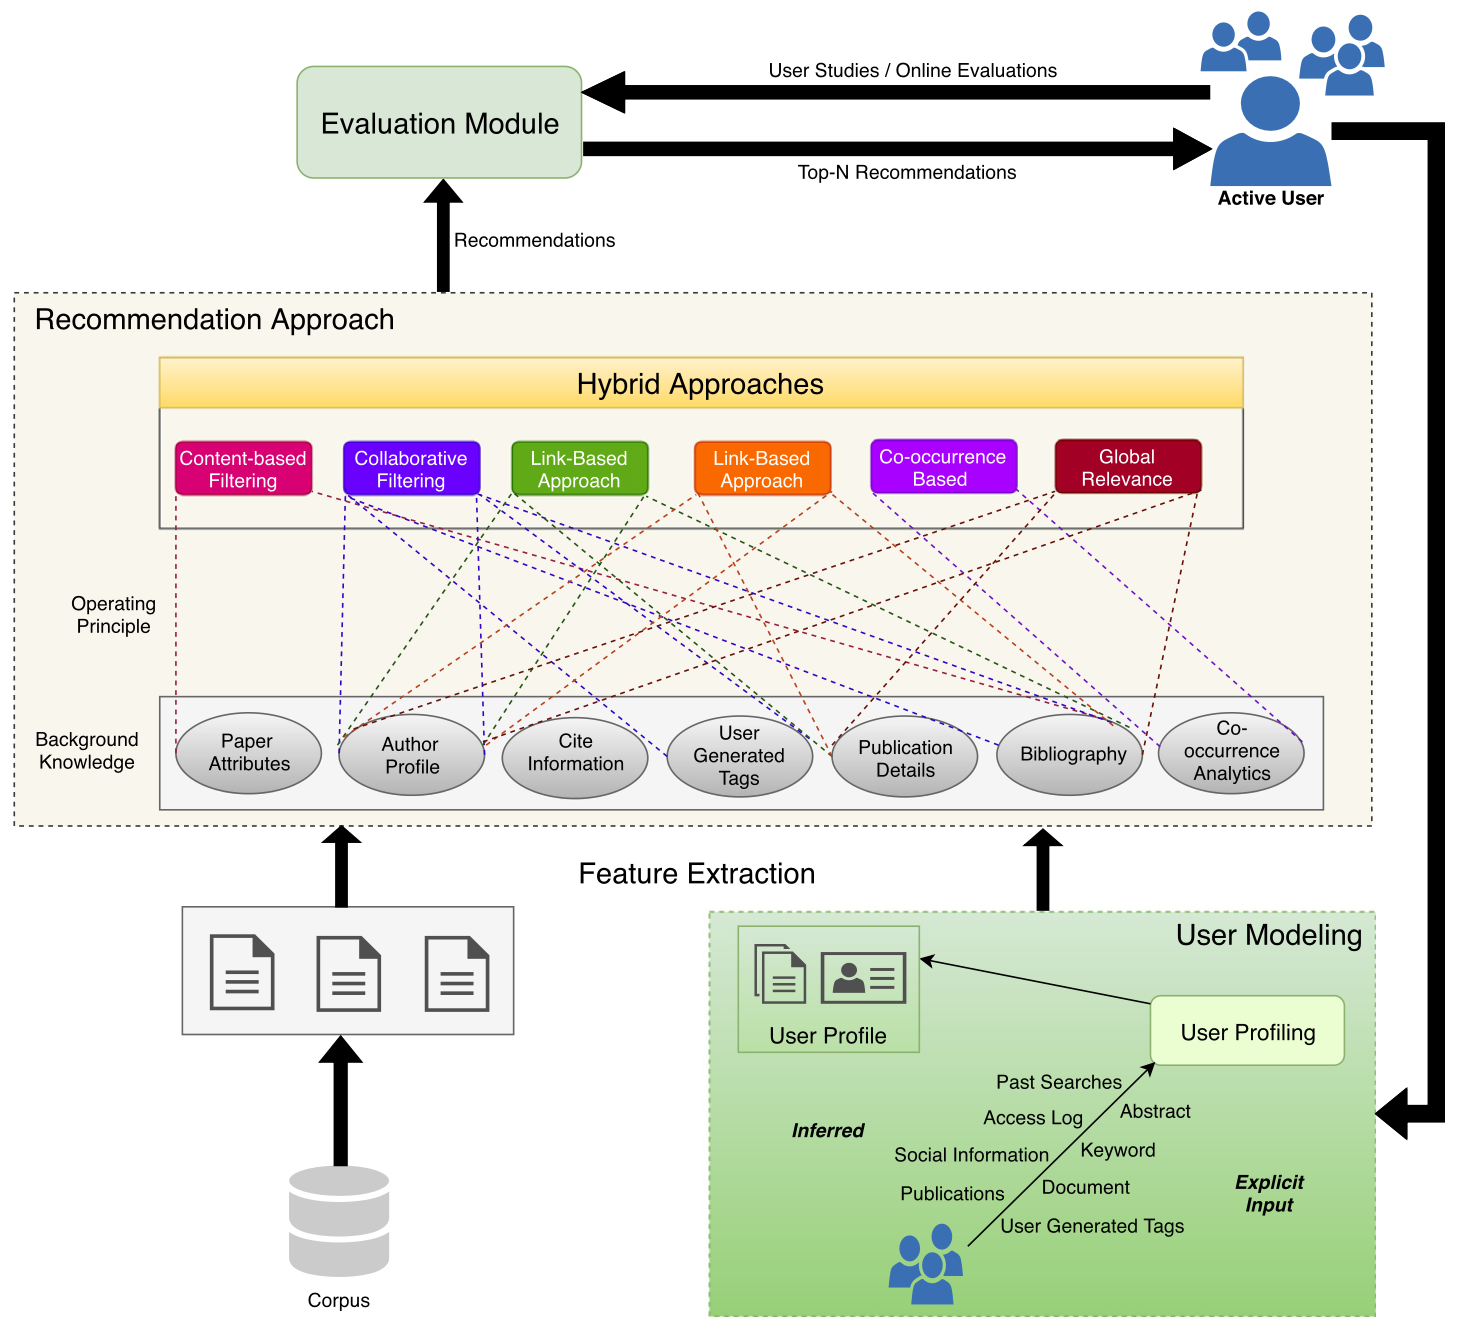
\includegraphics[width=0.7\textwidth]{figures/literature-review/general-architecture-rprs.png}
     \rule{35em}{0.5pt}
    \caption{General architecture of Research Paper Recommendation System (\textcite{Sharma2023})}
 \label{fig:general-architecture-rprs}
\end{figure}

The authors highlight the dominance of \gls{cbf} techniques, which rely on textual similarity between papers and user profiles, and discuss how \gls{cf} leverages peer preferences to improve recommendations.
Hybrid methods, which integrate multiple approaches, are presented as a solution to address the limitations of individual techniques, such as over-specialization in \gls{cbf} and data sparsity in \gls{cf}.
The study also identifies critical challenges, including the lack of standard datasets for benchmarking, insufficient evaluation metrics for dimensions like novelty and serendipity, and the difficulty of scaling algorithms to handle real-world, large-scale datasets.
Furthermore, the paper underscores the need for more sophisticated evaluation frameworks and advanced computational models, such as \gls{dl}, to improve the efficacy and scalability of research paper recommender systems.

\textcite{Jagadishwari2023} proposed a methodology for recommending academic collaborators using a combination of citation analysis and academic influence metrics.
Their work highlights the importance of identifying suitable collaborators to enhance research productivity and addresses the challenges posed by the vast volume of academic data.
The system utilizes the DBLP dataset \cite{Ley2002}, focusing on core computer science publications from 2017 to 2019, and incorporates citation count and influential citation metrics to assess academic influence.
The methodology involves preprocessing the dataset to eliminate irrelevant data, computing an Academic Level Index (ALI) using three different formulae, and then calculating a Research Score (R score) based on ALI and domain-specific publication metrics.
The R score serves as the basis for ranking scholars and identifying potential collaborators.
Three variations of the R score computation are tested, and the study concludes that the third formula (R3 Score) yields the most compatible recommendations by minimizing differences between the scores of the target scholar and recommended collaborators.
The system's results are visualized using graphs and compared across the three scoring methods, demonstrating that R3 Score provides the most precise matches.
The authors suggest future research could include additional factors like geographic location and funding status, as well as expanding the dataset to other academic disciplines.

\textcite{Zhang2023} provide a comprehensive review of scholarly recommendation systems, highlighting their evolution, methodologies, applications, and challenges.
These systems play a crucial role in academia, assisting researchers in identifying relevant literature, potential collaborators, conferences, journals, datasets, and grant opportunities.
The study identifies \gls{cbf} as the most widely used technique, particularly for literature recommendations, whereas \gls{cf} is more prevalent in conference and collaborator recommenders.
Hybrid approaches, which combine \gls{cbf} and \gls{cf}, are also discussed as a promising direction for improving recommendation accuracy and diversity.
The paper evaluates 225 publications across various SRS domains, showing that literature and collaborator recommendation systems dominate the field, while systems for datasets and grants are underexplored.
It notes the limited adoption of deep learning methods in scholarly recommendation systems and emphasizes the need for better integration of user feedback mechanisms to enhance system personalization and effectiveness.
Furthermore, the study highlights the challenges of scalability, data sparsity, and the cold start problem in existing systems.
Evaluation methods, including online and offline metrics, are examined, with offline evaluations being the most common.
In its conclusion, this work stresses the importance of developing unified frameworks that integrate diverse methodologies and leverage advances in \gls{ai} to address current limitations.
It also calls for more research into underrepresented areas like dataset and grant recommendation systems, advocating for user-centric designs that prioritize usability and practical application.

\textcite{Du2022} propose a novel model called ACR-ANE to enhance the recommendation of academic collaborators by integrating network topology and multi-type scholar attributes.
The study addresses the limitations of existing approaches, which often consider only local network structures or singular attribute types, and introduces non-local neighbors to capture stronger academic relationships.
Non-local neighbors are determined through biased random walks and frequency filtering, allowing the model to identify significant connections beyond immediate collaborators.
The methodology incorporates six scholarly attributes-academic age, research interests, publication count, average citations, number of collaborators, and H-index, into a scholar attribute matrix.
These attributes, combined with network structure, are encoded using a deep auto-encoder to generate low-dimensional embeddings that preserve both local and global academic network characteristics.
The model establishes a new multi-type relational network by integrating non-local neighbors and attribute-based proximity, which enriches the representation of academic relationships.
The framework of ACR-ANE is shown in Fig.~\ref{fig:acr-ane}.

\begin{figure}[htbp]
    \centering
 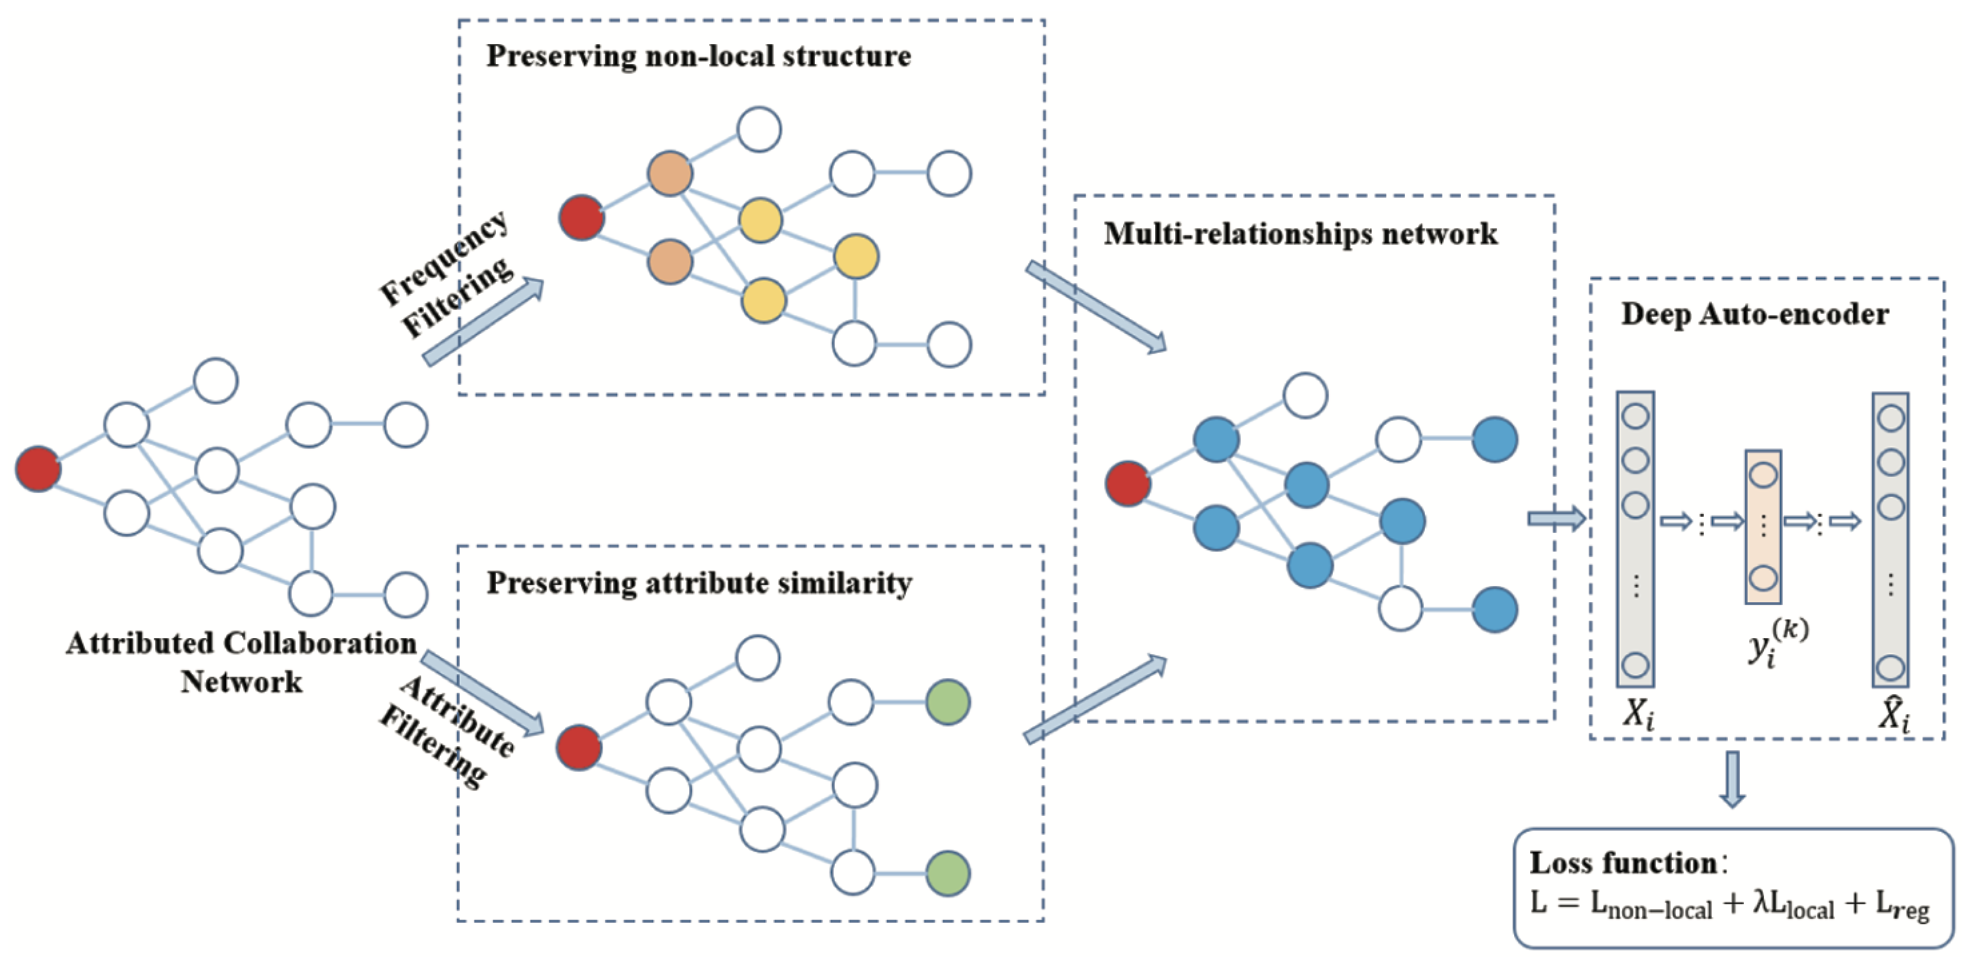
\includegraphics[width=0.8\textwidth]{figures/literature-review/academic-collaborator-recommendation-framework.png}
     \rule{35em}{0.5pt}
    \caption{The framework of ACR-ANE model. (\textcite{Du2022})}
 \label{fig:acr-ane}
\end{figure}

Extensive experiments conducted on two real-world datasets, Aminer and APS, demonstrate the superior performance of ACR-ANE in comparison to baseline models such as DeepWalk, TADW, SDNE, and ACNE.
The results highlight the effectiveness of combining network structure and scholar attributes for collaborator recommendation.
However, the study acknowledges its limitation in handling dynamic networks and suggests future work on incorporating temporal factors to reflect evolving academic collaborations.

\textcite{Zhu2022} explore the application of \glspl{gnn} to recommend research collaborators in the academic domain.
The study focuses on leveraging dynamic and temporal aspects of research networks, addressing the challenge of identifying suitable collaborators in a rapidly evolving academic landscape.
The authors utilize data from the MEDLINE database and implement two \gls{gnn}-based models, GraphSAGE and \gls{tgn}, to capture both static and temporal dependencies among researchers.
GraphSAGE employs an inductive approach that generates embeddings for unseen nodes by aggregating neighbor features, making it suitable for large and dynamic graphs.
\gls{tgn} extends this by incorporating temporal elements, using a message-passing mechanism to update node embeddings based on time-stamped interactions.
These models are compared against baseline methods, including the transductive LightGCN and a \gls{gbc}.
The study is divided into two experimental scenarios: automatic evaluations using \gls{auc} and average precision metrics, and external evaluations based on user ratings collected via a web-based application.
Results indicate that \gls{tgn} outperforms other methods in handling temporal dynamics and inductive tasks, particularly when using publication titles as node features.
While GraphSAGE exhibits strong performance for static embeddings, \gls{tgn} demonstrates superior capability in predicting future collaborations by integrating time-sensitive relationships.
The authors acknowledge limitations such as the small sample size in external evaluations and the reliance on static node features for some tests.
They propose future enhancements, including the integration of distribution-based representations for nodes to better manage uncertainty and improve predictive modeling.

\subsection*{Retrieval-Augmented Recommender Systems}\label{sec:retrieval-augmented-recommender-systems-in-research-field}

As described in Sec.~\ref{sec:retrieval-augmented-generation} and according to \textcite{Deldjoo2024}, \gls{rag} leverages the integration of retrieval systems and generative models to produce highly relevant and context-aware recommendations.
This approach stores knowledge externally, allowing dynamic updates and reducing the risk of hallucinations by grounding outputs in retrieved data.
By minimizing the need for extensive model parameters, \gls{rag} improves efficiency and makes complex tasks, such as generating personalized explanations, more feasible.
However, its effectiveness is strictly linked to the quality and relevance of the retrieved information, making it reliant on robust retrieval systems and well-curated external knowledge bases.
Additionally, the integration of retrieval and generation components introduces complexity and potential computational overhead, especially in real-time applications.
Despite these challenges, \gls{rag} offers a powerful framework for enhancing the accuracy and adaptability of modern recommender systems.

For example, \textcite{Banerjee2024} propose an approach to improve tourism recommender systems by integrating sustainability considerations into the recommendation process.
The authors leverage \gls{rag} to enhance \glspl{llm} for generating recommendations, focusing on sustainable city trips in Europe.
Their main innovation is the incorporation of a sustainability metric during the \gls{rag} pipeline's prompt augmentation phase, called Sustainability Augmented Reranking (SAR).
Fig.~\ref{fig:sar-enhanced-recommendation} illustrates the SAR-enhanced recommendation process, which adjusts the traditional \gls{rag} pipeline by including a sustainability metric based on city popularity and seasonal demand.

\begin{figure}[htbp]
    \centering
    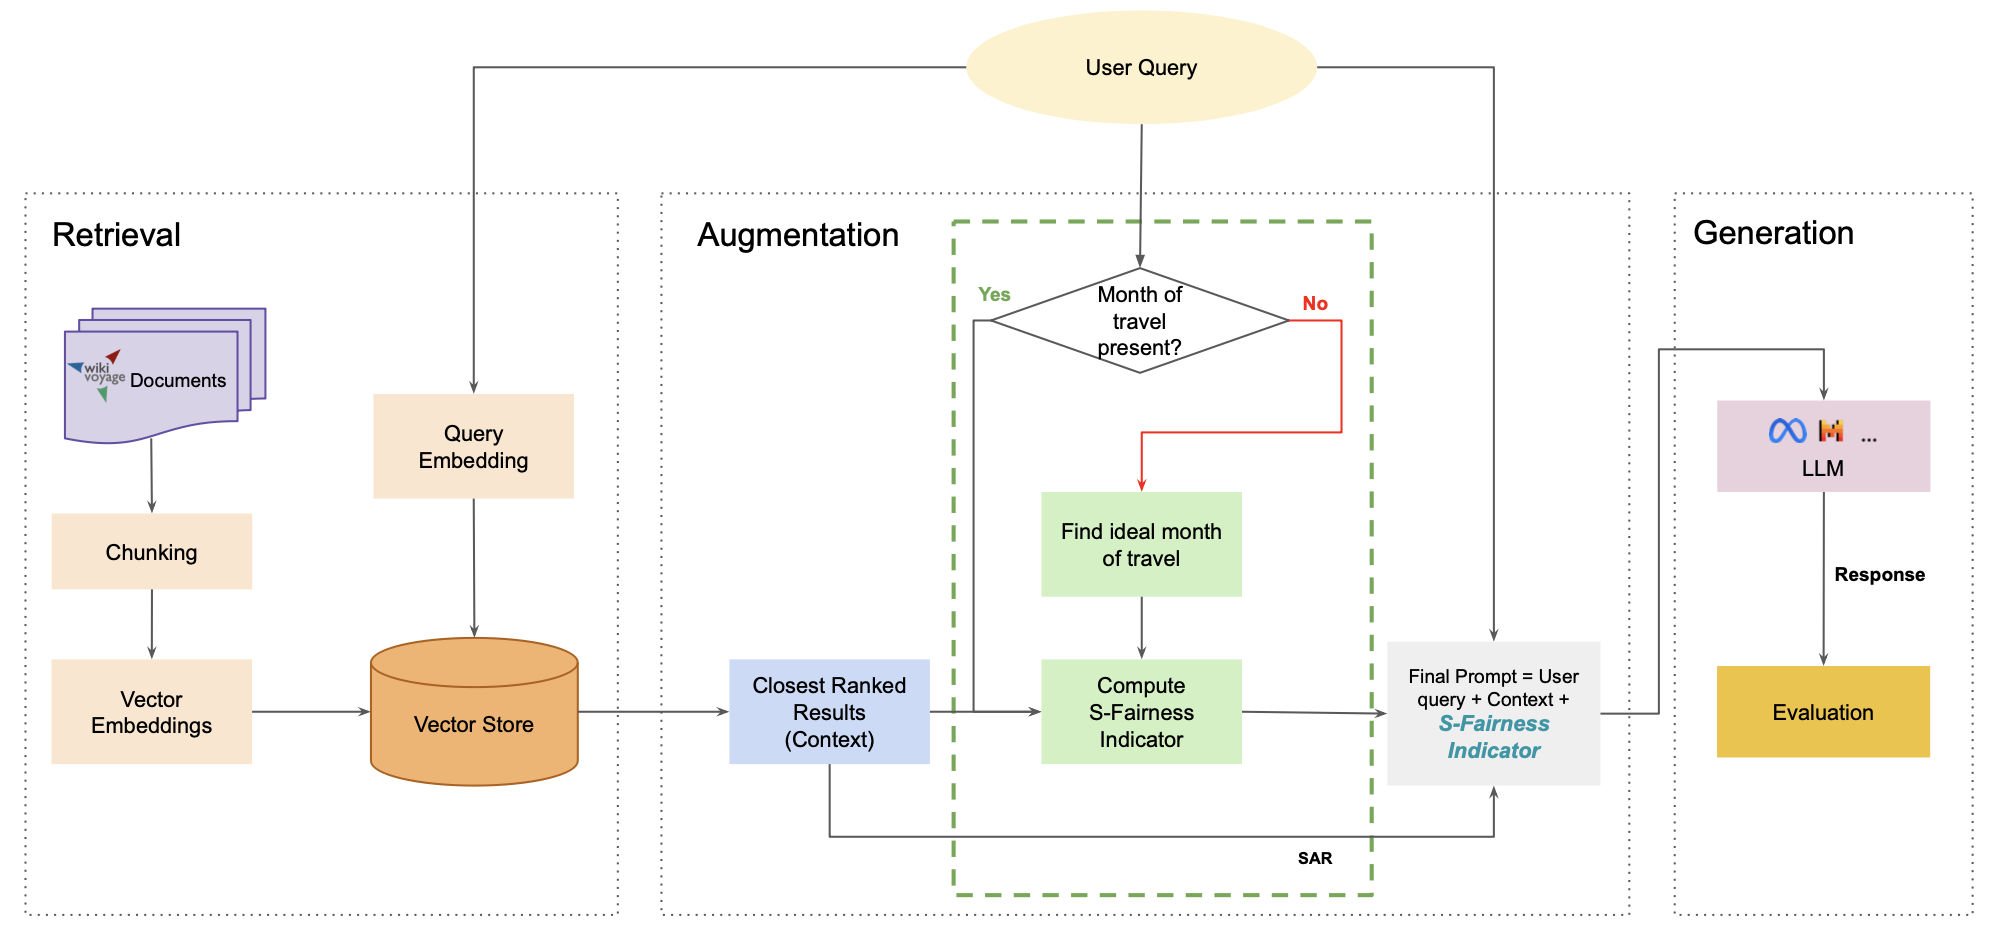
\includegraphics[width=0.8\textwidth]{figures/literature-review/rag-tourism.png}
    \rule{35em}{0.5pt}
    \caption{SAR-enhanced recommendation process (\textcite{Banerjee2024})}
 \label{fig:sar-enhanced-recommendation}
\end{figure}

The SAR enhancement adjusts the traditional \gls{rag} process by including a sustainability metric based on city popularity and seasonal demand.
This metric helps the system prioritize recommendations that align with sustainability principles, such as promoting destinations with lower tourism pressure during certain months.
By leveraging data from sources like Wikivoyage\footnote{\url{https://www.wikivoyage.org}} and Tripadvisor\footnote{\url{https://www.tripadvisor.com}}, the system calculates popularity and seasonality indices to inform the SAR metric, ensuring that recommendations balance user preferences with environmental and societal considerations.
Using open-source \glspl{llm}, such as Llama-3.1-Instruct-8B and Mistral-Instruct-7B, the study demonstrates that SAR-enhanced recommendations perform equal to or better than baseline models (without SAR) in terms of quality and sustainability.
The approach reduces common issues in \gls{llm}-based TRS, like hallucinations, and supports a multi-stakeholder perspective by addressing the needs of users, local communities, and environmental sustainability.

Another example is \gls{ramo}, a system designed to enhance Massive Open Online Courses (MOOCs) recommendations by addressing the ``cold start'' problem common in recommender systems \cite{Rao2024}.
Traditional course recommendation systems often struggle with new users due to the absence of historical data.
\gls{ramo} tackles this limitation by leveraging a \gls{rag} pipeline integrated with \gls{llm}.
In \gls{ramo}, the \gls{rag} framework combines two key components: a retriever and a generator.
The retriever accesses a pre-built knowledge base of course data, such as Coursera's publicly available dataset, and retrieves relevant information based on user queries.
The retrieved content is used to augment the prompts provided to the generator, ensuring responses are contextually relevant and precise.
This setup enables \gls{ramo} to generate personalized course recommendations even when little or no user-specific information is available, thereby overcoming the cold start issue.
The \gls{ramo} system workflow is shown in Fig.~\ref{fig:ramo-system-workflow}.

\begin{figure}[htbp]
    \centering
    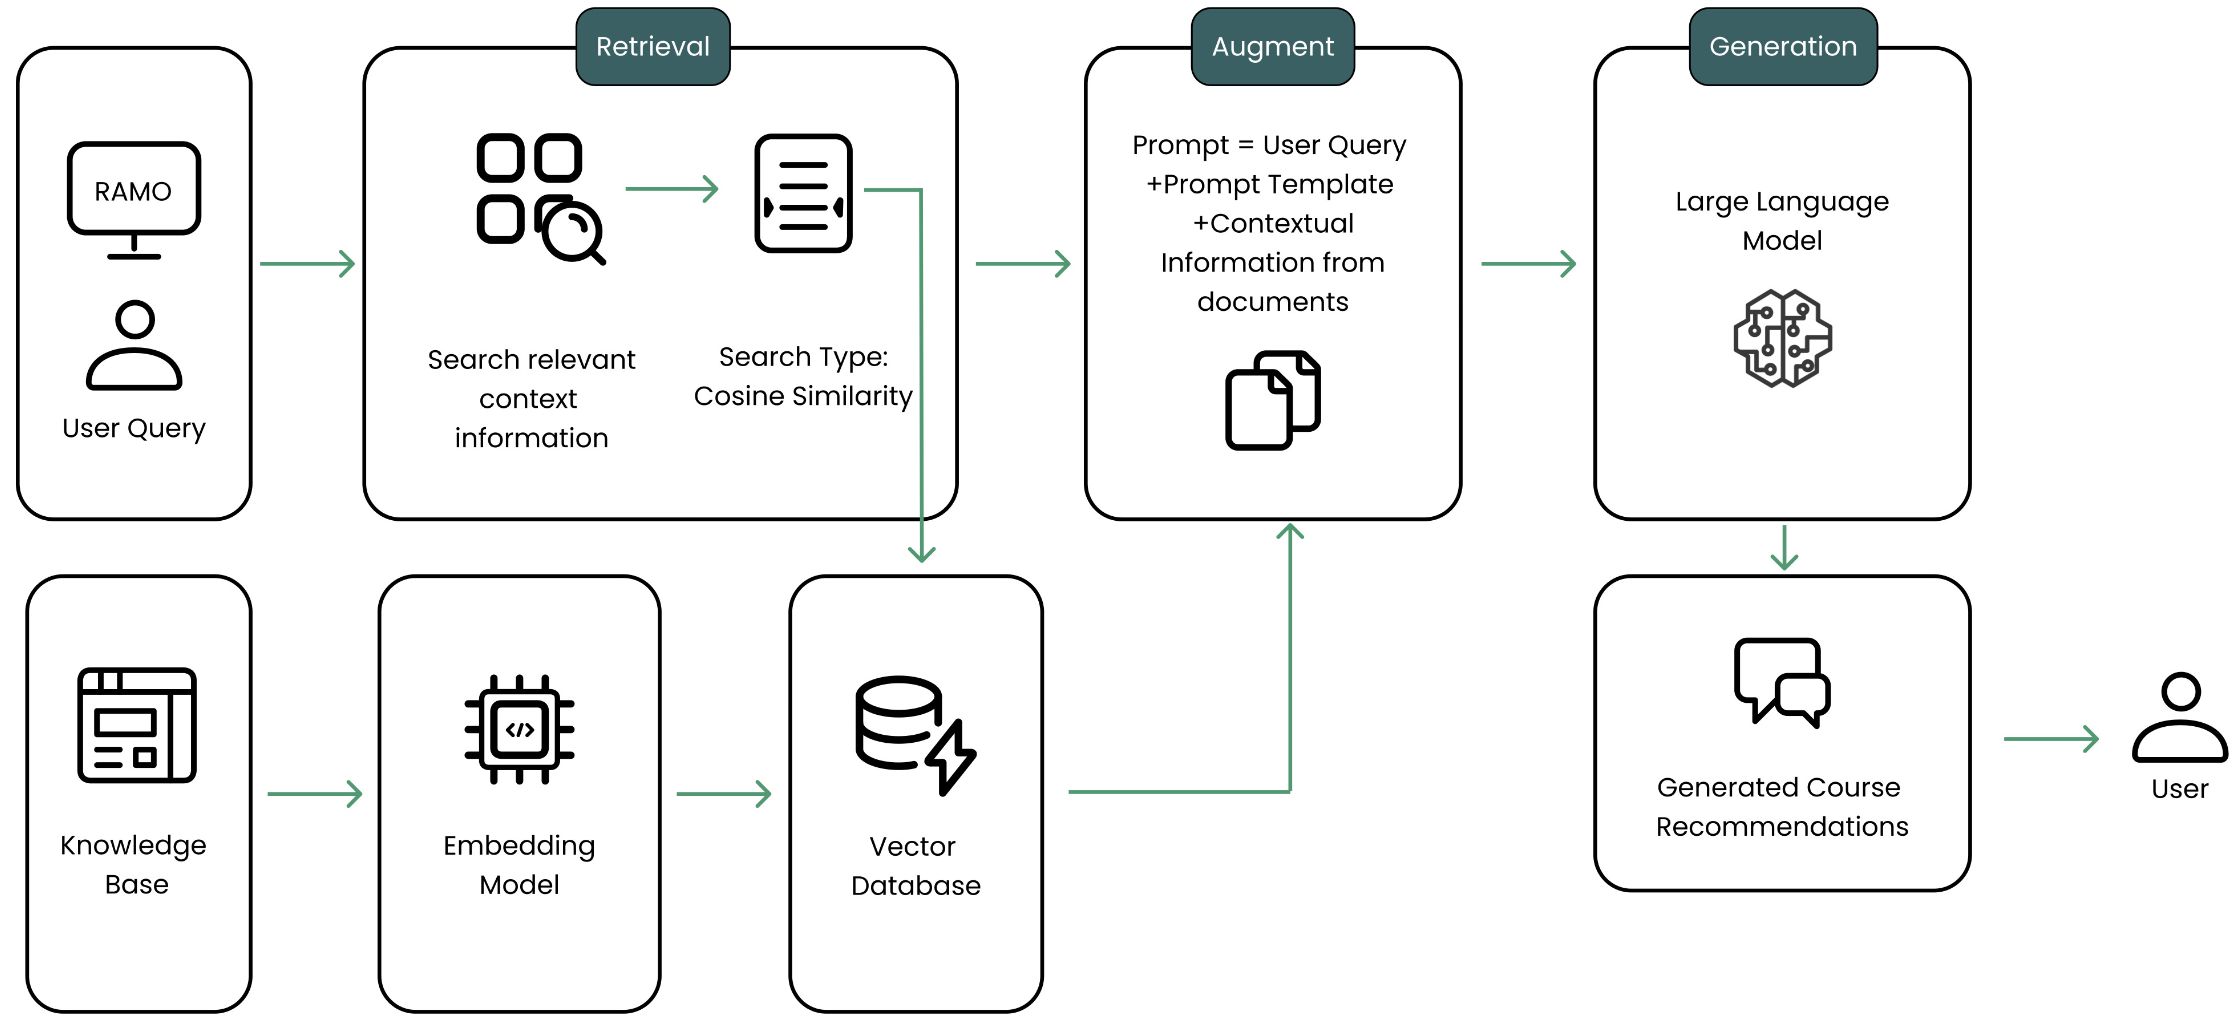
\includegraphics[width=0.8\textwidth]{figures/literature-review/ramo.png}
    \rule{35em}{0.5pt}
    \caption{The \gls{ramo} System workflow (\textcite{Rao2024})}
 \label{fig:ramo-system-workflow}
\end{figure}

The system utilizes advanced text embedding techniques to store and retrieve course data efficiently, employing models like OpenAI's text-embedding-ada-002 for embedding generation.
The final recommendations are produced by GPT-3.5 Turbo, selected for its cost-efficiency and performance, allowing dynamic, conversational interaction with users.
The paper evaluates \gls{ramo} by comparing its performance to traditional systems and standard \gls{llm}-based recommenders without \gls{rag}.
Results show that the \gls{rag}-enhanced system delivers more personalized and flexible recommendations, particularly in scenarios requiring personalized suggestions or dealing with general queries from new users.
The integration of \gls{rag} also ensures that the recommendations align closely with user needs by dynamically retrieving and incorporating domain-specific knowledge.

\textcite{DiPalma2023} explore the integration of \glspl{llm} into recommender systems to address challenges like cold-start problems, data sparsity, and adaptability to unseen data.
While traditional methods such as \gls{cf}, matrix factorization, and \gls{cbf} are effective in structured domains, they struggle in dynamic environments.
In contrast, \glspl{llm} leverage vast pre-trained knowledge, enabling them to generate meaningful recommendations even in novel scenarios.
To combine these strengths, the paper proposes a Retrieval-Augmented Recommender System that integrates retrieval-based and generative models to enhance accuracy and explainability.
This framework allows recommender systems to retrieve relevant external knowledge while using \glspl{llm} for improved reasoning and contextual adaptation.
The study examines \glspl{llm} in two roles: at the higher level, powering conversational \gls{ai} for personalized recommendations, and at the lower level, refining recommendation strategies through knowledge retrieval and generation.
Evaluating GPT-3.5 on MovieLens100K and Facebook Books datasets, the study compares its performance with state-of-the-art baselines using accuracy metrics such as nDCG, HR, and MAP.
GPT-3.5 performs competitively, particularly excelling in book recommendations due to its extensive pretraining on book-related data.
In movie recommendations, its performance is slightly lower than top models, highlighting the need for fine-tuning or retrieval augmentation.
Despite its potential, several challenges arise in integrating \glspl{llm} into recommender systems.
The cold-start problem persists, as effectiveness varies by dataset and domain.
Hallucination remains an issue, with models generating inaccurate or non-existent recommendations.
Popularity bias limits diversity, and the lack of real-time updates prevents awareness of newly introduced items.
Additionally, the black-box nature of \glspl{llm} raises concerns about explainability compared to traditional, more interpretable recommender systems.

\textcite{Wu2024} addresses the challenge of long-tail recommendation, where traditional \gls{cf}-based recommender systems struggle due to data sparsity and imbalance.
While \glspl{llm} have demonstrated strong reasoning capabilities, they typically rely on item semantics and fail to capture collaborative user-item interaction patterns, leading to misaligned recommendations.
To overcome this limitation, the authors introduce CoRAL, a collaborative retrieval-augmented \gls{llm} framework that integrates collaborative evidence into \gls{llm} prompts, ensuring alignment with real-world user-item interactions.
CoRAL enhances recommendation performance by retrieving minimal-sufficient collaborative information through a reinforcement learning-based retrieval policy, optimizing the inclusion of relevant interactions while minimizing unnecessary data that could distract the \gls{llm}.
The framework formulates long-tail recommendation as a sequential decision-making problem, where the retrieval policy dynamically selects user-item interactions to support the \gls{llm}'s reasoning process.
Experimental evaluations on Amazon product datasets demonstrate that CoRAL significantly outperforms both traditional \gls{cf} methods and standard \gls{llm}-based recommendation approaches, achieving superior accuracy in predicting user preferences.
The study highlights the importance of integrating collaborative knowledge with \glspl{llm} for long-tail recommendation and suggests reinforcement learning as a viable approach for optimizing retrieval-augmented recommendations.